\chapter{Compensador analógico} \chapterlabel{Informe/6-CompensadorAnalogico} \label{cap:Compensador Analogico}

En este capítulo se analiza la dinámica de la planta que se desea controlar y se utilizan distintas estrategias de análisis y compensación para conseguir que el sistema de levitación presente el comportamiento deseado. 

Como se mencionó en la sección \ref{sec_modelo_estados}, el fenómeno de levitación magnética presenta un comportamiento inestable. Es por ello que se debe implementar un lazo de control que logre estabilizar el sistema. Se propone una estrategia de control mediante la implementación de un compensador ($G_c$) dentro de un lazo de control interno y luego, un compensador ($G_{ext}$) en un lazo de control externo para mejorar su respuesta temporal. En la figura \ref{fig:diag-en-bloques-comp} se muestra un diagrama en bloques genérico de la estrategia compensación planteada.

\begin{figure}[H]
	\centering
	\scalebox{0.8}{\tikzset{%
	buffer/.style={
		draw,
		shape border rotate=270,
		regular polygon,
		regular polygon sides=3,
		fill=blue!20,
		node distance=2cm,
		minimum height=4em
	}
}

\tikzstyle{block} = [draw, fill=blue!20, rectangle, 
minimum height=2.5em, minimum width=3em]

%Acá se define eñ diagrama en bloques completo
\begin{tikzpicture}[auto, node distance=1cm,>=latex']
	% We start by placing the blocks
	\node [input, name=input] {};
	\node [buffer, right=of input](F){F};
	\node [sum, right of=F, node distance=1.5cm] (suma_externa) {+};
	\node [block, right=of suma_externa] (externo) {$G_{ext}$};
	\node [sum, right=of externo] (suma_interna) {+};
	\node[block, right=of suma_interna] (interno) {$G_c$};
	\node [block, right=of interno] (gil) {$G_{IL}$};
	\node [block, right=of gil] (planta) {$G_p$};
	\node [block, below=of interno] (realimentacion_interna) {$H_{estim}$};
	
	\node [block, below=2cm of externo] (realimentacion_externa) {$H_{estim}$};
%	
%	\node [block, right of=suma] (amplificador) {$A(s)$};
	\node [output, right of=planta, node distance=3cm] (output) {};
%	\node [block, below of=amplificador] (realimentacion) {$H(s)$};
%	
%	
%	% Once the nodes are placed, connecting them is easy. 
	\draw [draw,->] (input) -- node[pos=0.2]{$V_{y_{ref}}$} (F);
	\draw [draw,->] (F) -- node[pos=0.9]{$+$}(suma_externa);
	\draw [draw,->] (suma_externa) -- (externo);
	\draw [draw,->] (externo) -- node[pos=0.95]{$+$} (suma_interna);
	\draw [draw,->] (suma_interna) -- (interno);
	\draw [draw,->] (interno) -- (gil);
	\draw [draw,->] (gil) -- (planta);
	\draw [draw,->] (planta) -- node[name=y]{$Y_g$} (output);
%	\draw [draw,->] (amplificador) -- node[name=y]{$V_{deriv}$} (output);
	\draw [->] (y) |- (realimentacion_interna);
	\draw [->] (realimentacion_interna) -| node[pos=0.25]{$V_{estim}$}  node[pos=0.99]{$-$} (suma_interna);
	\draw [->] (y) |- (realimentacion_externa);
	\draw [->] (realimentacion_externa) -| node[pos=0.25]{$V_{estim}$} node[pos=0.99]{$-$} (suma_externa);
\end{tikzpicture}}
	\caption{Diagrama en bloques de estrategia de compensación propuesta.}	\label{fig:diag-en-bloques-comp}
\end{figure}

\section{Diseño del lazo de realimentación interno}

En esta sección se diseña el control del lazo de realimentación interno, que está compuesto por las etapas mostradas en la figura \ref{fig:diag-interno}. Donde $G_c$ corresponde a la transferencia del compensador que se desea diseñar, $G_{IL}$ a la transferencia del controlador de corriente, $G_p$ a la transferencia de la planta y $H_{estim}$ a la del estimador de distancia de entrehierro.


\begin{figure}[H]
	\centering
	\tikzset{%
	buffer/.style={
		draw,
		shape border rotate=270,
		regular polygon,
		regular polygon sides=3,
		fill=blue!20,
		node distance=2cm,
		minimum height=4em
	}
}

\tikzstyle{block} = [draw, fill=blue!20, rectangle, 
minimum height=2.5em, minimum width=3em]

%Acá se define eñ diagrama en bloques completo
\begin{tikzpicture}[auto, node distance=1.5cm,>=latex']
	% We start by placing the blocks
	\node [input, name=input] {};
	\node [sum, right of=input, node distance=1.5cm] (suma_interna) {+};
	\node[block, right=of suma_interna] (interno) {$G_c$};
	\node [block, right=of interno] (gil) {$G_{IL}$};
	\node [block, right=of gil] (planta) {$G_p$};
	\node [block, below=of gil] (realimentacion_interna) {$H_{estim}$};
	
	
%	\node [block, right of=suma] (amplificador) {$A(s)$};
	\node [output, right of=planta, node distance=3cm] (output) {};
%	\node [block, below of=amplificador] (realimentacion) {$H(s)$};
%	
%	
%	% Once the nodes are placed, connecting them is easy. 
%	\draw [draw,->] (input) -- node[pos=0.2]{$V_{y_{ref}}$} (F);
	\draw [draw,->] (input) -- node[pos=0.2]{$V_{ref_c}$} node[pos=0.9]{$+$}(suma_interna);

	\draw [draw,->] (suma_interna) -- node{$Ve_{int}$} (interno);
	\draw [draw,->] (interno) -- node{$V_{IL{ref}}$} (gil);
	\draw [draw,->] (gil) -- node{$I_L$} (planta);
	\draw [draw,->] (planta) -- node[name=y]{$Y_g$} (output);
%	\draw [draw,->] (amplificador) -- node[name=y]{$V_{deriv}$} (output);
	\draw [->] (y) |- (realimentacion_interna);
	\draw [->] (realimentacion_interna) -| node[pos=0.25]{$V_{estim}$}  node[pos=0.99]{$-$} (suma_interna);
%	\draw [->] (y) |- (realimentacion_externa);
%	\draw [->] (realimentacion_externa) -| node[pos=0.25]{$V_{estim}$} node[pos=0.99]{-} (suma_externa);
\end{tikzpicture}
	\caption{Diagrama en bloques del lazo de compensación interno.}	\label{fig:diag-interno}
\end{figure}

Las funciones transferencia de cada bloque del diagrama \ref{fig:diag-interno} están dadas por:

\begin{equation*}
	G_{IL}(s) =\frac{I_L[A]}{V_{IL_{ref}}[V]}=\frac{6}{1+\frac{s}{12.17}}
\end{equation*}

\begin{equation*} 
	G_{p}(M,s)=\frac{Y_g[m]}{I_L[A]}=-\sqrt{\frac{30}{M}}*\frac{1.201}{s^{2}-4900}
\end{equation*}

\begin{equation*} 
	H_{estim}(s)=\frac{V_{estim}[V]}{Y_{g}[m]}=\frac{259.6}{(1+\frac{s}{1\:kr/s})}
\end{equation*}

La transferencia de lazo cerrado ($TLC_{interna}$) del diagrama \ref{fig:diag-interno} queda definida como:

\begin{equation}
	TLC_{interna}=\frac{Y_g[m]}{V_{ref_c}[V]}=\frac{G_c*G_{IL}*G_p}{1+G_c*G_{IL}*G_p*H_{estim}}
\end{equation}

A continuación se analiza la estabilidad de la planta considerando una masa $M=30\:kg$ y se diseña el bloque del compensador interno $G_c(s)$ para lograr estabilizarla. Luego, se verificará la estabilidad con este mismo compensador para una masa $M=1\:kg$, que corresponde a la mínima con la que trabaja el sistema.

\subsection{Análisis de estabilidad}

Para realizar el análisis de estabilidad se parte de las transferencias de la planta $G_{p}(s)$ para una masa de $30\:kg$, del controlador de corriente $G_{IL}(s)$ y del lazo de realimentación $H_{estim}(s)$. A partir de ellas se obtiene la transferencia a lazo abierto $GH_T(s)$ de la expresión \ref{eq_GT2}, que presenta cuatro polos, con uno de ellos con parte real positiva en $70\:r/s$.

\begin{equation*}
	GH_T(s)=G_{p}(s)*G_{iL}(s)*H_{estim}(s) 
\end{equation*}

\begin{equation} \label{eq_GT2}
		GH_T(s)=\frac{0.38}{(1-(\frac{s}{70\:r/s})^2)(1+\frac{s}{12.17\:r/s })(1+\frac{s}{1\:kr/s}) }	
\end{equation}


Para comenzar el análisis se considera un compensador $G_c=K$, donde K es una constante positiva. Por lo tanto, se plantea la transferencia de lazo abierto teniendo en cuenta el compensador:

\begin{equation} \label{eq_GT3}
	G_c*GH_T(s)=\frac{K*0.38}{(1-(\frac{s}{70\:r/s})^2)(1+\frac{s}{12.17\:r/s })(1+\frac{s}{1\:kr/s}) }	
\end{equation}

Utilizando la transferencia de la ecuación \ref{eq_GT3}, con $K=1$, se  grafican los diagramas de Bode y de Nyquist y, a partir de ellos, se analiza la estabilidad. Estos se muestran en las figuras \ref{fig:Diag_Bode_lazo_abierto_30kg} y \ref{fig:Diag_Nyquist_lazo_abierto_30kg} respectivamente.

\begin{figure}[H]
	\centering
	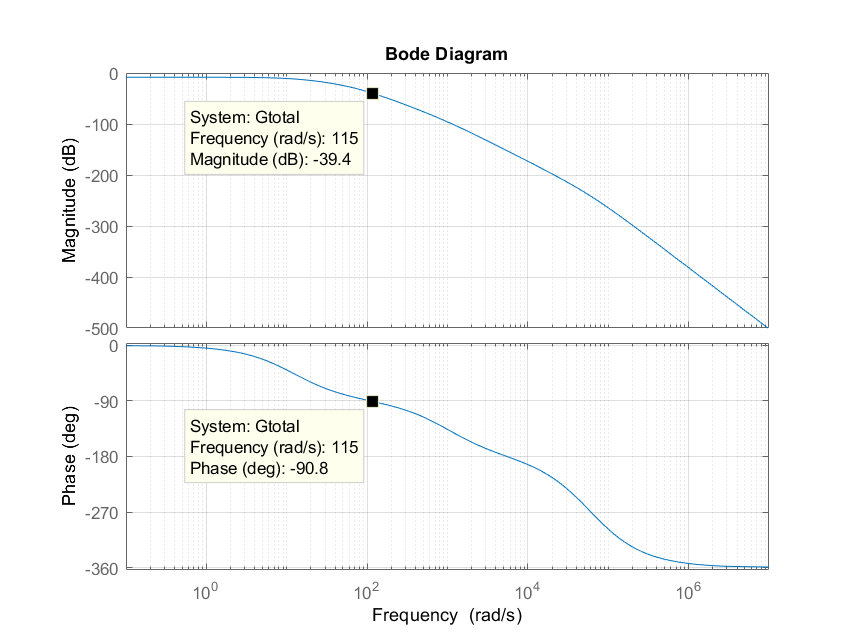
\includegraphics[scale=0.8]{bode_planta_30kg.png}
	\caption{Diagrama de Bode de lazo abierto $G_c*GH_T$ con $M=\:30 kg$.}
	\label{fig:Diag_Bode_lazo_abierto_30kg}
\end{figure}

\begin{figure}[H]
	\centering
	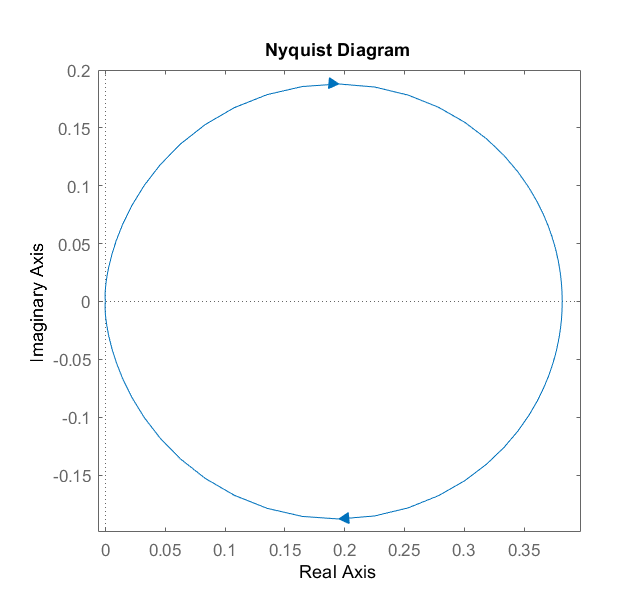
\includegraphics[scale=0.6]{nyquist_planta_30kg.png}
	\caption{Diagrama de Nyquist de $G_c*GH_T$ con $M=30\:kg$.}
	\label{fig:Diag_Nyquist_lazo_abierto_30kg}
\end{figure}


%\noindent Con la transferencia de la ecuación  \ref{eq_GT2} se  grafica el diagrama de Bode  en la figura \ref{fig:Diag_Bode_lazo_abierto_30kg}. El criterio de estabilidad de Bode dice que para determinar la estabilidad de un sistema en un diagrama de Bode se debe observar si la magnitud es mayor a 0dB antes de que la fase alcance -180°. En este caso nuestro sistema es de no mínima fase... \colorbox{red}{ver si dejamos esto o vamos directo a nyquist}

Como la transferencia de la planta $GH_T$ tiene un polo en el semiplano derecho del plano ``S'' no es posible determinar su estabilidad por medio del diagrama de Bode. Por lo tanto, se analiza la estabilidad por medio del criterio de Nyquist.

Como se observa en el diagrama en bloques de la figura \ref{fig:diag-interno}, para compensar al sistema se planteó una realimentación negativa. Por lo tanto, para analizar su estabilidad según Nyquist se deben determinar la cantidad de giros (N) de $G_c*GH_T$ alrededor del punto $-1+j0$ en la figura \ref{fig:Diag_Nyquist_lazo_abierto_30kg} y la cantidad de polos (P) en el semiplano derecho de la función transferencia $G_c*GH_T$. El sistema resultará estable si se cumple la condición \ref{eq_condicion_Nyquist}, donde Z representa la cantidad de ceros en el semiplano derecho de $1+G_c*GH_T(s)$.

\begin{equation}\label{eq_condicion_Nyquist}
	Z=N+P=0
\end{equation}


Debido a que $GH_T$ tiene un polo en el semiplano derecho ($P=1$) y no hay giros alrededor del punto $-1+j0$ ($N=0$), resulta que $Z=1$. Por lo tanto, la transferencia de lazo cerrado ($TLC_{interna}$) presenta un comportamiento inestable. En la figura \ref{fig:Diag_Nyquist_lazo_abierto_30kg} se puede observar que no existe ningún valor de $K>0$ que haga que el contorno de $G_c*GH_T$ rodee el punto $-1+j0$. Por lo tanto, se propone implementar un compensador con $K<0$, para invertir el contorno de $G_c*GH_T$. Esto resulta equivalente a considerar $K>0$ y usar realimentación positiva en el lazo de control interno. De esta forma se obtiene el diagrama en bloques de la figura \ref{fig:diag-interno_realimentacion_positiva}.


\begin{figure}[H]
	\centering
	\tikzset{%
	buffer/.style={
		draw,
		shape border rotate=270,
		regular polygon,
		regular polygon sides=3,
		fill=blue!20,
		node distance=2cm,
		minimum height=4em
	}
}

\tikzstyle{block} = [draw, fill=blue!20, rectangle, 
minimum height=2.5em, minimum width=3em]

%Acá se define eñ diagrama en bloques completo
\begin{tikzpicture}[auto, node distance=1.5cm,>=latex']
	% We start by placing the blocks
	\node [input, name=input] {};
	\node [sum, right of=input, node distance=1.5cm] (suma_interna) {+};
	\node[block, right=of suma_interna] (interno) {$G_c$};
	\node [block, right=of interno] (gil) {$G_{IL}$};
	\node [block, right=of gil] (planta) {$G_p$};
	\node [block, below=of gil] (realimentacion_interna) {$H_{estim}$};
	
	
%	\node [block, right of=suma] (amplificador) {$A(s)$};
	\node [output, right of=planta, node distance=3cm] (output) {};
%	\node [block, below of=amplificador] (realimentacion) {$H(s)$};
%	
%	
%	% Once the nodes are placed, connecting them is easy. 
%	\draw [draw,->] (input) -- node[pos=0.2]{$V_{y_{ref}}$} (F);
	\draw [draw,->] (input) -- node[pos=0.2]{$Vref2$} node[pos=0.9]{+}(suma_interna);

	\draw [draw,->] (suma_interna) -- node{$Ve2??$} (interno);
	\draw [draw,->] (interno) -- node{$V_{IL{ref}}$} (gil);
	\draw [draw,->] (gil) -- node{$I_L$} (planta);
	\draw [draw,->] (planta) -- node[name=y]{$Y_g$} (output);
%	\draw [draw,->] (amplificador) -- node[name=y]{$V_{deriv}$} (output);
	\draw [->] (y) |- (realimentacion_interna);
	\draw [->] (realimentacion_interna) -| node[pos=0.25]{$V_{estim}$}  node[pos=0.99]{-} (suma_interna);
%	\draw [->] (y) |- (realimentacion_externa);
%	\draw [->] (realimentacion_externa) -| node[pos=0.25]{$V_{estim}$} node[pos=0.99]{-} (suma_externa);
\end{tikzpicture}
	\caption{Diagrama en bloques del lazo de compensación interno considerando realimentación positiva.}	\label{fig:diag-interno_realimentacion_positiva}
\end{figure}


La realimentación positiva se genera al sumar la señal $V_{estim}$ con la señal de entrada del sistema. La transferencia de lazo cerrado del diagrama en bloques ahora se define como:

\begin{equation}
	TLC_{interna}=\frac{Y_g[m]}{V_{ref_c}[V]}=\frac{G_c*G_{IL}*G_p}{1-G_c*G_{IL}*G_p*H_{estim}}
\end{equation}

Siguiendo el criterio de estabilidad de Nyquist, al utilizar realimentación positiva, la cantidad de giros (N) debe analizarse alrededor del punto $1+j0$. Si estos son en sentido horario, N será positivo, caso contrario será negativo. Al variar el valor de K, es posible hacer que el punto $1+j0$ quede contenido en la zona 1 o en la zona 2 de la figura \ref{fig:nyquist-con-zonas}. 

\begin{figure}[H]
	\centering
	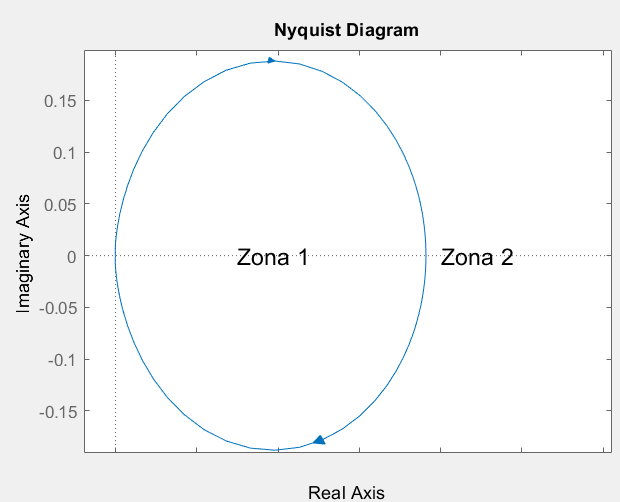
\includegraphics[scale=0.7]{nyquist_con_zonas.png}
	\caption{Diagrama de Nyquist con zonas marcadas.}	
	\label{fig:nyquist-con-zonas}
\end{figure}

Si el punto queda dentro de la zona 1, el número de giros es $N=1$. Por lo tanto, se plantea:

\begin{equation*}
	Z = N + P = 2
\end{equation*}


Si el punto queda dentro de la zona 2, el número de giros es $N=0$. Por lo tanto, se plantea:

\begin{equation*}
	Z = N + P = 1
\end{equation*}

Debido a que en ambas zonas Z resulta mayor que cero, el sistema realimentado no puede ser estabilizado con ningún valor de K. Para lograrlo se debe implementar un compensador $G_c$ que sea capaz de generar una zona en el diagrama de Nyquist donde exista un giro alrededor de $1 + j0$ en sentido antihorario de forma tal que $N=-1$ y resulte $Z=0$. Para ello, es necesario aumentar la fase para que pueda superar el valor de 0$\mathrm{{}^\circ}$. Para que esto se cumpla, el diagrama de Nyquist debe tener una forma como la  mostrada en la figura \ref{fig:nyquist-deseado-analog}.

\begin{figure}[H]
	\centering
	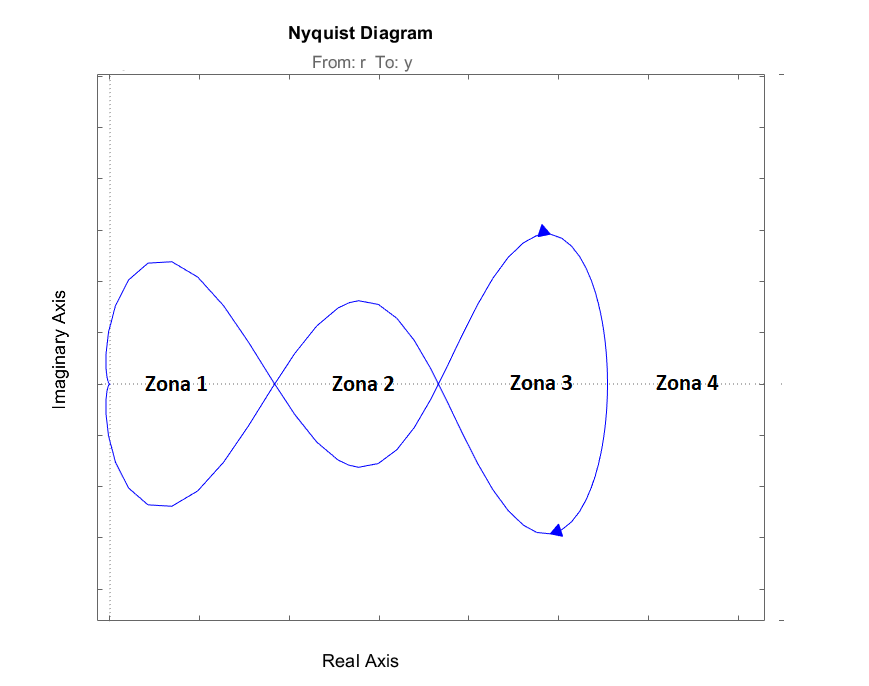
\includegraphics[scale=0.7]{Nyquist-deseado-analog.png}
	\caption{Forma del diagrama de Nyquist deseado.}
	\label{fig:nyquist-deseado-analog}
\end{figure}

De esta manera se identifican cuatro zonas en las que puede estar ubicado el punto $1+j0$. Sin embargo, solo en la zona 2 se genera un giro en sentido antihorario ($N=-1$) como es deseado, por lo que resulta:

\begin{equation*}
	Z = N + P = 0
\end{equation*}

%Para lograr el comportamiento del sistema como en la figura 	\ref{fig:nyquist-deseado-analog} se debe tener en cuenta que el m\'{o}dulo de la transferencia de lazo abierto en el primer cruce de la fase por 0$\mathrm{{}^\circ}$ debe ser mayor a $0\:dB$ y, en el segundo cruce, menor. Para ello, se propone implementar un compensador por adelanto de fase.

A continuación se diseñará el compensador $G_c$ para lograr que el diagrama de Nyquist tenga la forma deseada y así, estabilizar el sistema.


\subsection{Diseño de compensador}

Para lograr el comportamiento del sistema como en la figura 	\ref{fig:nyquist-deseado-analog} se utilizará una estrategia de compensación por adelanto de fase. Esta consiste en observar el diagrama de bode de la figura \ref{fig:Diag_Bode_lazo_abierto_30kg} y elegir una frecuencia en la que se desee aumentar la fase para lograr la estabilidad. Se debe tener en cuenta que el módulo de la transferencia de lazo abierto en el primer cruce de la fase por 0$\mathrm{{}^\circ}$ debe ser mayor a $0\:dB$ y, en el segundo cruce, menor. 

De esta forma, al observar la figura \ref{fig:Diag_Bode_lazo_abierto_30kg} se decide generar un adelanto de fase de por lo menos 100° en la frecuencia $200\:r/s$. Esto se logra mediante el uso de un compensador compuesto por dos redes de adelanto de fase de 65$\mathrm{{}^\circ}$ cada una. 

Una red de adelanto de fase está compuesta por un polo ($W_p$) y un cero ($W_c$), de manera que el cero se encuentra a una frecuencia menor que el polo, permitiendo un aumento de fase a la frecuencia deseada $W_0$. Su transferencia es la siguiente:

\begin{equation} \label{eq_tf_adelanto}
	G_{af}(s)=\alpha*\frac{(s + W_c)}{(s + W_p)}
\end{equation}

\noindent De esta forma, las ecuaciones de dise\~{n}o resultan:

\begin{equation*}
	\begin{aligned}
		&W_0 =200\:r/s\\
		&{\varphi }_{max} =65\textrm{°}\\
		&\alpha =\frac{1+sen({\varphi }_{max})}{1-sen{(\varphi }_{max})}=20.346\\
		&W_c =\frac{W_0}{\sqrt{\alpha }}=\ 44.3\:r/s\\
		&W_p =\sqrt{\alpha }*W_0=902.1\: r/s\\
	\end{aligned}
\end{equation*} 
\noindent Finalmente, agregando una ganancia K y considerando las dos redes de adelanto de fase, se llega a la transferencia del controlador:

\begin{equation}  
	G_c(s)=K*{[20.346*\frac{(s+44.3)}{(s+902.1)}]}^2
	\label{eq:transferencia-del-compensador}
\end{equation} 

\noindent En la figura \ref{fig:bode-analog-compensado-para-k-1} se muestra el diagrama de bode de ${GH}_T*G_c$ con $K=1$. Se puede observar que se logró aumentar la fase de la manera deseada. Para finalizar el diseño del compensador se debe elegir un valor apropiado para la ganancia $K$.

La ganancia $K$ puede adoptar valores desde $15.7\:dB$ hasta $35.5\:dB$ aproximadamente. Al considerar que el sistema debe soportar una masa variable entre $1\:kg$ y $30\:kg$, y que la ganancia de la transferencia de la planta para $1\:kg$ es de $5.5$ veces ($14\:dB$) mayor que para $30\:kg$, se debe adoptar una ganancia del compensador que mantenga la estabilidad para estos dos casos. Es decir, la ganancia mínima es de $15.7\:dB$ y la máxima es de $35.5\:dB - 14\:dB = 21.5\:dB$. Por lo tanto, se elige que el cruce por cero de la ganancia se encuentre ahora en $88\:r/s$, lo que significa que $K=20\:dB\ \equiv \ 10\: veces$. Se elige este valor para priorizar la estabilidad para el caso de masa máxima, con la desventaja de que se obtiene un menor margen de fase para el caso de masa mínima. \colorbox{red}{capaz esto lo sacamos}


\begin{figure}[H]
	\centering
	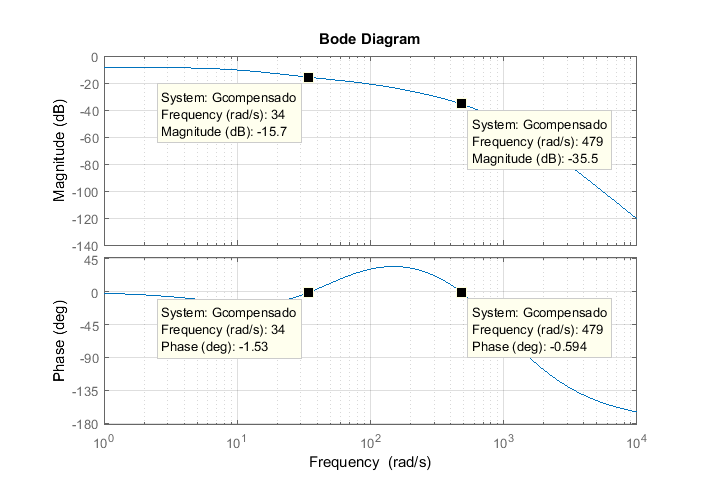
\includegraphics[scale=0.85]{Bode-k-1-M-30.png}
	\caption{Diagrama de Bode de $GH_T*G_c$ para $K=1$ y $M=30\:kg$.}
	\label{fig:bode-analog-compensado-para-k-1}
\end{figure}

\noindent En la figura \ref{fig:bode-analog-compensado-para-k-10} se muestra el diagrama de Bode al considerar la ganancia del compensador. En ella se puede observar que se  cumple con el criterio de estabilidad, puesto que en el primer cruce por 0°, la magnitud es mayor a 0 dB y en el segundo cruce, menor. Además, en la figura \ref{fig:nyquist-analog-para-k-10} se grafica el diagrama de Nyquist para el sistema con el compensador. En él se puede ver que el punto $1+j0$ queda dentro de la zona en la que $N=-1$, que resulta en $Z=0$.

\begin{figure}[H]
	\centering
	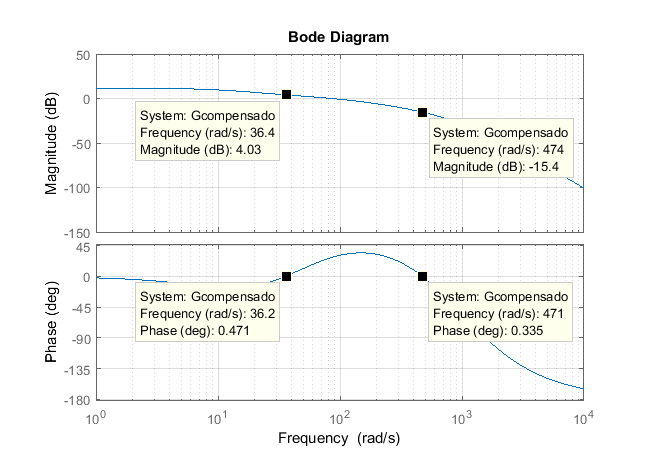
\includegraphics[scale=0.8]{Bode-k-10-M-30.png}
	\caption{Diagrama de Bode de $GH_{T}*G_c$ para $K=10$ y $M=30\:kg$.}
	\label{fig:bode-analog-compensado-para-k-10}
\end{figure}

\begin{figure}[H]
	\centering
	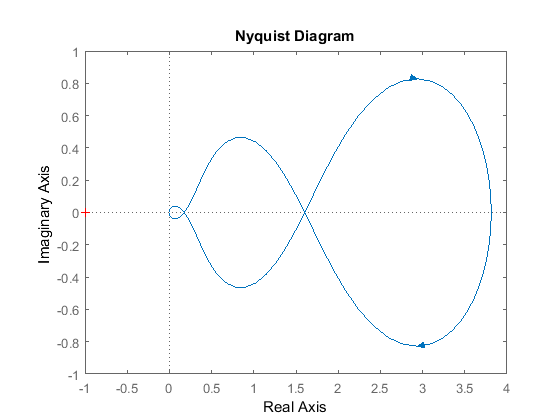
\includegraphics[scale=0.8]{Nyquist-k-10-M-30.png}
	\caption{Diagrama de Nyquist de $GH_T*G_c$ para $K=\:10$ y $M=30\:kg$.}
	\label{fig:nyquist-analog-para-k-10}
\end{figure}


\subsection{Verificación de estabilidad con masa de 1 kg}

%\noindent Se verifica la estabilidad del sistema  para el caso en que la masa sea de $1\:kg$ con el compensador dise\~{n}ado para el caso de masa m\'{a}xima. Para ello, se analizan los diagramas de Bode y Nyquist mostrados en las figuras \ref{fig:bode-analog-para-M-1Kg} y \ref{fig:nyquist-analog-para-M-1Kg}. Adem\'{a}s, en la figura \ref{fig:respuesta-analog-al-escalon-para-M-1Kg} puede observarse la respuesta al escal\'{o}n. A partir de ellos, es posible verificar que el sistema resulta estable para todo el rango de masas en el que opera el sistema. 

\noindent Se verifica la estabilidad del sistema  para el caso en que la masa sea de $1\:kg$ con el compensador previamente diseñado. Para ello, se analizan los diagramas de Bode y Nyquist mostrados en las figuras \ref{fig:bode-analog-para-M-1Kg} y \ref{fig:nyquist-analog-para-M-1Kg}. A partir de ellos, es posible verificar que el sistema resulta estable para todo el rango de masas en el que opera el sistema. Sin embargo, se puede observar que el margen de fase es menor que 45°, por lo que el sistema puede presentar un transitorio con oscilaciones amortiguadas. A raiz de esto, se propone implementar un lazo de control externo que permita mejorar dicha respuesta.

\begin{figure}[H]
	\centering
	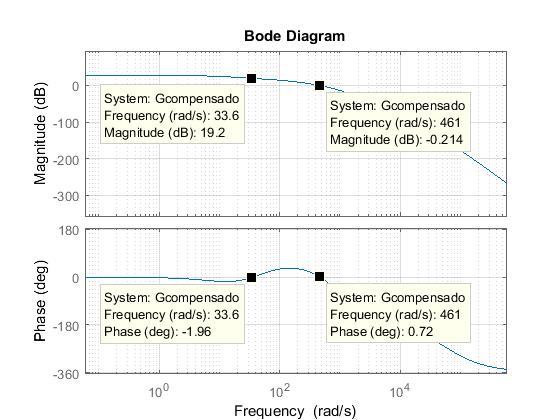
\includegraphics[scale=0.80]{bodecompensado1kg.png}
	\caption{Diagrama de Bode de $GH_T*G_c$ para $M=1\:kg$.}
	\label{fig:bode-analog-para-M-1Kg}
\end{figure}


\begin{figure}[H]
	\centering
	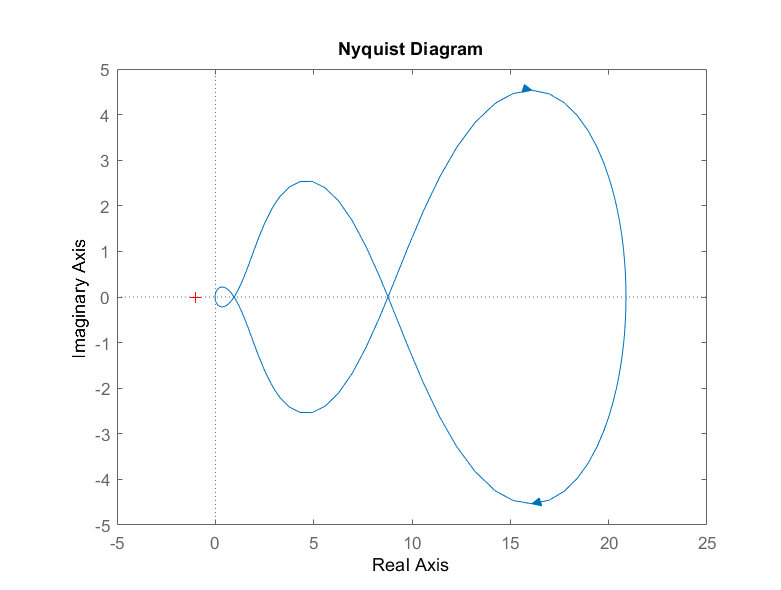
\includegraphics[scale=0.55]{nyquistcompensado1kg.png}
	\caption{Diagrama de Nyquist de $GH_T*G_c$ para $M=1\:kg$.}
	\label{fig:nyquist-analog-para-M-1Kg}
\end{figure}

%\begin{figure}[H]
%	\centering
%	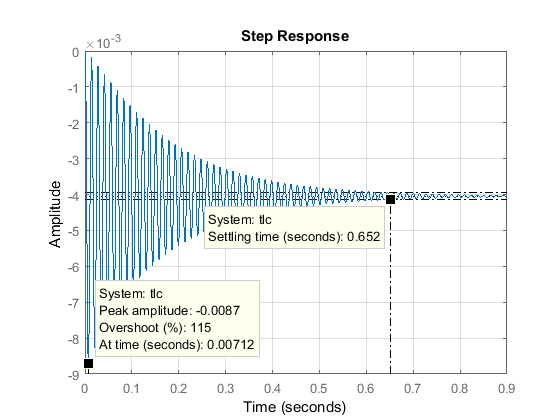
\includegraphics[scale=0.80]{rtaescaloncompensado1kg.png}
%	\caption{Respuesta al escalón para $M=1\:kg$.}
%	\label{fig:respuesta-analog-al-escalon-para-M-1Kg}
%\end{figure}

\subsection{Transferencia de lazo cerrado}


Finalmente se puede expresar la función transferencia del lazo de control interno como:
%
%-3.6301e05 (s+1000) (s+44.3)^2
%------------------------------------------------------------------
%(s+304.3) (s+115.6) (s^2 + 44.84s + 2588) (s^2 + 2352s + 1.498e06)


\begin{equation}
	TLC_{interna}(s)=\frac{Y_g}{V_{ref_c}}=\frac{G_c*G_{p}*G_{iL}}{1-G_c*G_{p}*G_{iL}*H_{estim}}
	%	\frac{-3.6301*}{den}
\end{equation}

Para el caso de trabajar con masa de $30\:kg$, la $TLC_{interna}$ resulta:

\begin{equation*}
	\resizebox{.99\hsize}{!}
	{
		$
		TLC_{interna}(s)=\frac{-3.6301*10^5(s+1000)(s+44.3)^2}{(s+304.3) (s+115.6) (s^2 + 44.84s + 2588) (s^2 + 2352s + 1.498*10^6)}
		$
	}
\end{equation*}


Para el caso de trabajar con masa de $1\:kg$, resulta:


\begin{equation*}
	\resizebox{.99\hsize}{!}
	{
		$
		TLC_{interna}(s)=\frac{-1.9883*10^6 (s+1000) (s+44.3)^2}{(s^2 + 88.82s + 2127) (s^2 + 18.19s + 2.117*10^5) (s^2 + 2709s + 2.142*10^6)}	
		$
	}
\end{equation*}



En las figuras \ref{fig:ubicacion_polos_y_ceros} y \ref{fig:ubicacion_polos_y_ceros_1kg} se muestra la ubicación de los polos y ceros de la $TLC_{interna}$ para el caso de masa de $30\:kg$ y $1\:kg$, respectivamente. En ellas se ve que todos se encuentran en el semiplano izquierdo. 

\begin{figure}[H]
	\centering
	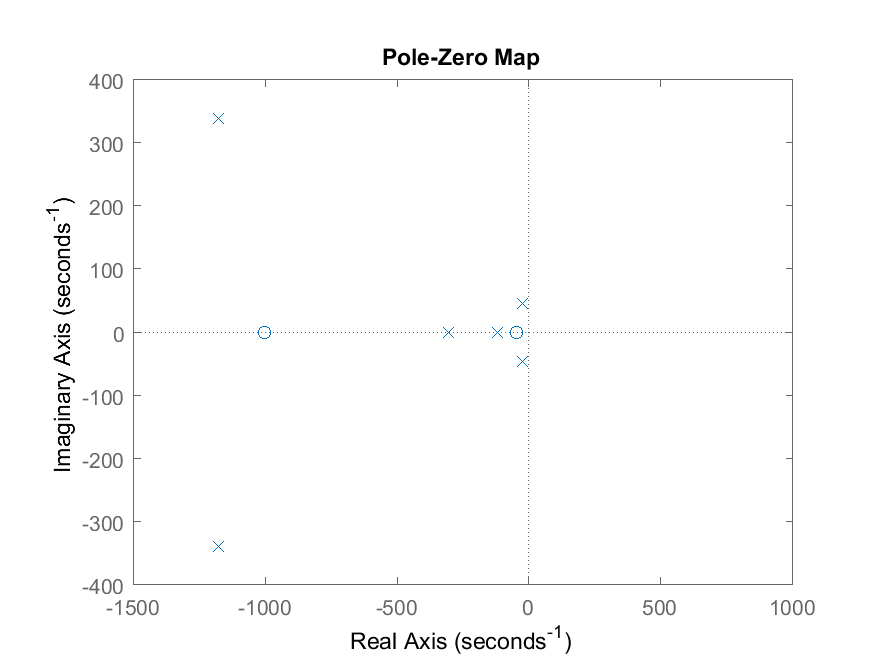
\includegraphics[scale=0.85]{ubicacion_polos_ceros.png}
	\caption{Ubicación de polos y ceros de la transferencia de lazo cerrado interna con $M=30\:kg$.}
	\label{fig:ubicacion_polos_y_ceros}
\end{figure}

\begin{figure}[H]
	\centering
	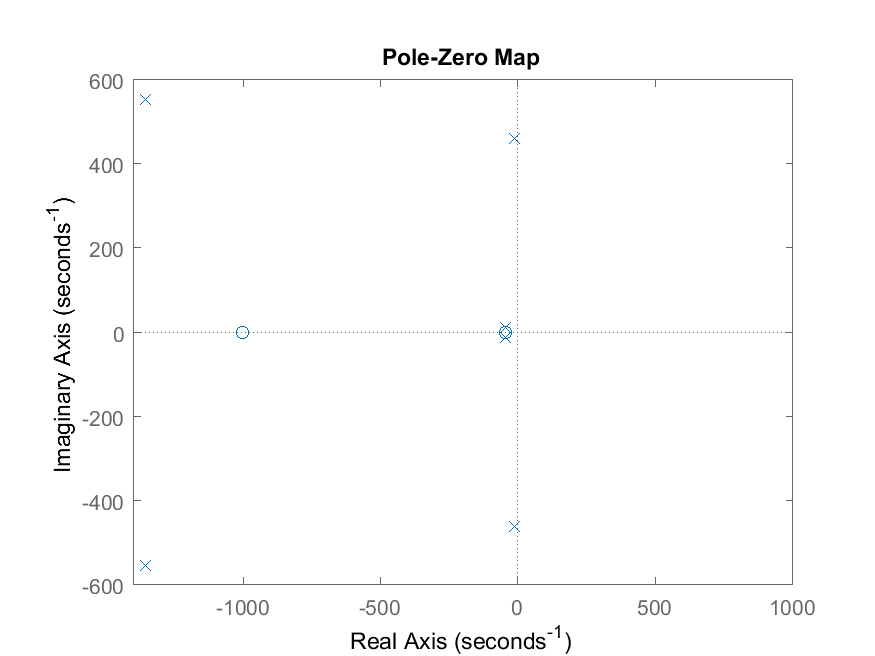
\includegraphics[scale=0.85]{ubicacion_polos_ceros_1kg.png}
	\caption{Ubicación de polos y ceros de la transferencia de lazo cerrado interna con $M=1\:kg$.}
	\label{fig:ubicacion_polos_y_ceros_1kg}
\end{figure}


Es importante notar que la ganancia de la transferencia de lazo cerrado en ambos casos es negativa. Esto debe tenerse en cuenta para el diseño del lazo de compensación externo.


%Por último se simuló la respuesta del sistema a un escalón de amplitud unitaria en la señal $V_{ref_c}$. La salida es un valor de distancia de entrehierro $Y_g$ en metros. En la figura \ref{fig:rta-escalon-k-10-m-30} se puede observar la respuesta al escalón del sistema con masa de $30\:kg$.
%
%\colorbox{red}{Ver como acomodar lo de la respuesta al escalon (y para 1kg tambien)}
%
%\begin{figure}[H]
%	\centering
%	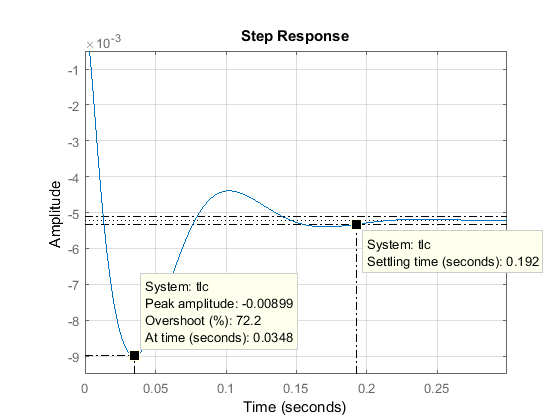
\includegraphics[scale=0.80]{Respuesta-al-escalon-K-10-M-30Kg.png}
%	\caption{Respuesta al escalón para $M=30\:kg$.}
%	\label{fig:rta-escalon-k-10-m-30}
%\end{figure}

\section{Diseño del lazo de realimentación externo}

\noindent Se plantea un lazo de realimentación externo como se muestra en la figura \ref{fig:diag-externo}. 

\begin{figure}[H]
	\centering
	\tikzset{%
	buffer/.style={
		draw,
		shape border rotate=270,
		regular polygon,
		regular polygon sides=3,
		fill=blue!20,
		node distance=2cm,
		minimum height=4em
	}
}

\tikzstyle{block} = [draw, fill=blue!20, rectangle, 
minimum height=2.5em, minimum width=3em]

%Acá se define eñ diagrama en bloques completo
\begin{tikzpicture}[auto, node distance=1.5cm,>=latex']
	% We start by placing the blocks
	\node [input, name=input] {};
	\node [buffer, right=of input](F){F};
	\node [sum, right of=F, node distance=1.5cm] (suma_interna) {+};
	\node [block, right=of suma_interna] (interno) {$G_{ext}$};
	\node [block, right=of interno] (tlc_interna) {$TLC_{interna}$};
	\node [block, below=of interno] (realimentacion_interna) {$H_{estim}$};
	
	
%	\node [block, right of=suma] (amplificador) {$A(s)$};
	\node [output, right of=tlc_interna, node distance=3cm] (output) {};
%	\node [block, below of=amplificador] (realimentacion) {$H(s)$};
%	
%	
%	% Once the nodes are placed, connecting them is easy. 
	\draw [draw,->] (input) -- node[pos=0.2]{$V_{y_{ref}}$} (F);
	\draw [draw,->] (F) --  node[pos=0.9]{$+$}(suma_interna);
	\draw [draw,->] (suma_interna) --node{$Ve_{ext}$} (interno);
	\draw [draw,->] (interno) -- node{$V_{ref_c}$} (tlc_interna);
	\draw [draw,->] (tlc_interna) -- node[name=y]{$Y_g$} (output);
%	\draw [draw,->] (amplificador) -- node[name=y]{$V_{deriv}$} (output);
	\draw [->] (y) |- (realimentacion_interna);
	\draw [->] (realimentacion_interna) -| node[pos=0.25]{$V_{estim}$}  node[pos=0.99]{$-$} (suma_interna);
%	\draw [->] (y) |- (realimentacion_externa);
%	\draw [->] (realimentacion_externa) -| node[pos=0.25]{$V_{estim}$} node[pos=0.99]{-} (suma_externa);
\end{tikzpicture}
	\caption{Diagrama en bloques del lazo de compensación externo.}	\label{fig:diag-externo}
\end{figure}

En el lazo de realimentación interno actúa el compensador por adelanto de fase previamente diseñado y, en el externo, un controlador del tipo integral. Esto permite suavizar la respuesta al escalón del sistema y eliminar el error en régimen permanente.


\noindent Para el an\'{a}lisis se considera como realimentaci\'{o}n: 

\[H_{estim}=\frac{V_{estim}}{Y_g[m]}= \frac{259.6}{(1 + \frac{s}{1\:k})
}\] 

\noindent La cadena de avance con masa de $30\:kg$ es:

\begin{equation} \label{eq_cadena_avance_integrador}
	G=TLC_{interna}(s)[M=30\:kg]*G_{ext}
\end{equation}

La transferencia a lazo abierto resulta:

\begin{equation} \label{eq_lazo_abierto_externo}
	GH_{externo}=TLC_{interna}(s)[M=30\:kg]*G_{ext}*H_{estim}
\end{equation}

Inicialmente se plantea un compensador del tipo integrador cuya transferencia es:
\begin{equation}
	G_{ext}= \frac{K_{int}}{s}
\end{equation}

El problema de este integrador es que presenta una ganancia infinita en continua. Por lo tanto, se propone implementar un compensador con un polo ($p_{int}$) en baja frecuencia, que actúe como integrador a las frecuencias de la planta, pero que tenga ganancia finita en continua. De esta forma, se decide ubicar el polo en $0.1\:rad/s$ y la transferencia a implementar resulta:

\begin{equation}
	G_{ext}=\frac{K_{int}}{1+\frac{s}{p_{int}}}=\frac{K_{int}}{1+\frac{s}{0.1\:r/s}}	
\end{equation}

Sin embargo, es importante tener en cuenta que la ubicación de un polo en baja frecuencia provoca que la cancelación del error en régimen permanente no sea completa.

%, pero de todas maneras sea pequeña en comparación con la distancia de separación.

%Debido a que no usamos un integrador ideal, la respuesta al escalón presentará un cierto error.
Para encontrar el valor adecuado de $K_{int}$ se grafica el lugar de raíces de la expresión \ref{eq_lazo_abierto_externo} considerando $K_{int}=1$. Este puede verse en la figura \ref{fig:lugar-de-raices-con-integrador-analog_inestable}.

\begin{figure}[H]
	\centering
	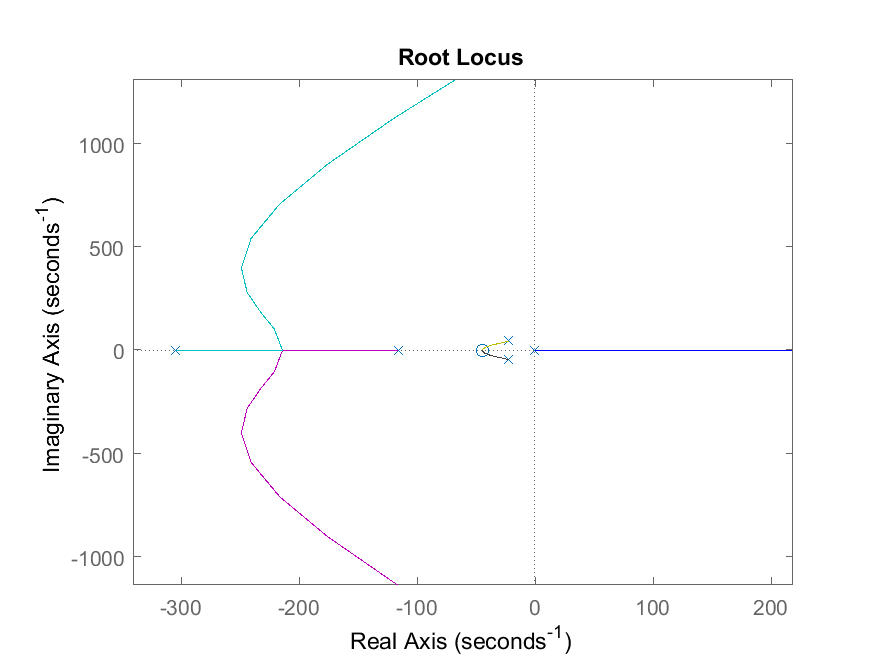
\includegraphics[scale=0.7]{rlocusconintegrador30kg_inestable.png}
	\caption{Lugar de raíces de $GH_{externo}$}.
	\label{fig:lugar-de-raices-con-integrador-analog_inestable}
\end{figure}

Para determinar el valor de ganancia $K_{int}$ máxima a partir del cual el polo se pasa al semiplano derecho, se realiza un acercamiento al lugar de raíces que se muestra en la figura \ref{fig:lugar-de-raices-con-integrador-analog_inestable_acercamiento}. 

\begin{figure}[H]
	\centering
	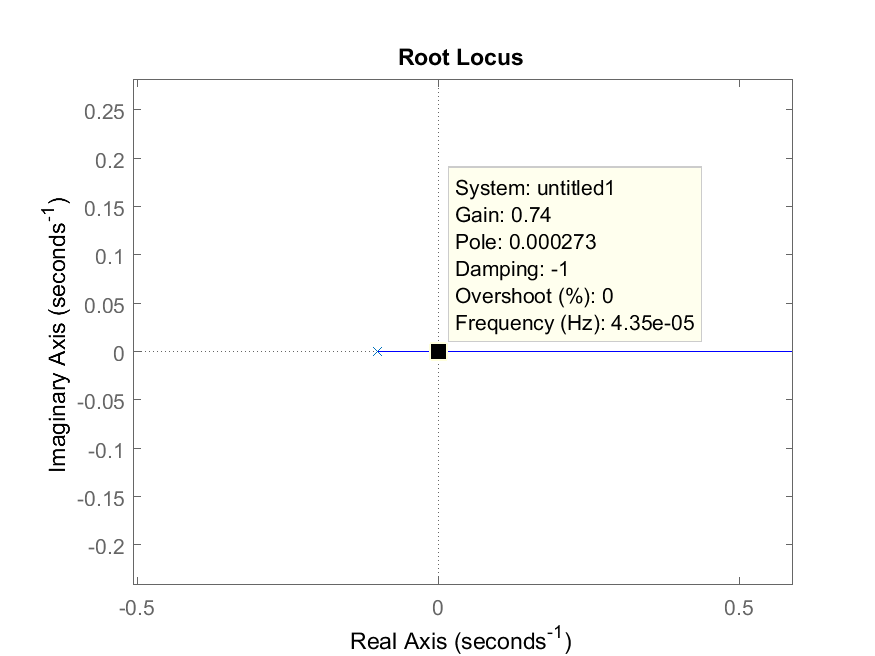
\includegraphics[scale=0.7]{rlocusconintegrador30kg_inestable_acercamiento.png}
	\caption{Acercamiento del lugar de raíces de $GH_{externo}$.}
	\label{fig:lugar-de-raices-con-integrador-analog_inestable_acercamiento}
\end{figure}

En la figura \ref{fig:lugar-de-raices-con-integrador-analog_inestable_acercamiento} se observa que el valor máximo de ganancia es $K_{int}=0.74$. Si bien el sistema resultaría estable para valores menores a este, su respuesta temporal sería demasiado lenta. 

Por lo tanto, se propone utilizar realimentación positiva en el diagrama en bloques de la figura \ref{fig:diag-externo}, obteniendo así el que se muestra la figura \ref{fig:diag-externo_real_positiva}. De esta forma, el polo de baja frecuencia cambia el sentido de desplazamiento y el lugar de raíces resulta como se muestra en la \ref{fig:lugar-de-raices-con-integrador-analog}.


\begin{figure}[H]
	\centering
	\tikzset{%
	buffer/.style={
		draw,
		shape border rotate=270,
		regular polygon,
		regular polygon sides=3,
		fill=blue!20,
		node distance=2cm,
		minimum height=4em
	}
}

\tikzstyle{block} = [draw, fill=blue!20, rectangle, 
minimum height=2.5em, minimum width=3em]

%Acá se define eñ diagrama en bloques completo
\begin{tikzpicture}[auto, node distance=1.5cm,>=latex']
	% We start by placing the blocks
	\node [input, name=input] {};
	\node [buffer, right=of input](F){F};
	\node [sum, right of=F, node distance=1.5cm] (suma_interna) {+};
	\node [block, right=of suma_interna] (interno) {$G_{ext}$};
	\node [block, right=of interno] (tlc_interna) {$TLC_{interna}$};
	\node [block, below=of interno] (realimentacion_interna) {$H_{estim}$};
	
	
%	\node [block, right of=suma] (amplificador) {$A(s)$};
	\node [output, right of=tlc_interna, node distance=3cm] (output) {};
%	\node [block, below of=amplificador] (realimentacion) {$H(s)$};
%	
%	
%	% Once the nodes are placed, connecting them is easy. 
	\draw [draw,->] (input) -- node[pos=0.2]{$V_{y_{ref}}$} (F);
	\draw [draw,->] (F) --  node[pos=0.9]{$+$}(suma_interna);
	\draw [draw,->] (suma_interna) -- node{$Ve_{ext}$} (interno);
	\draw [draw,->] (interno) -- node{$V_{ref_c}$} (tlc_interna);
	\draw [draw,->] (tlc_interna) -- node[name=y]{$Y_g$} (output);
%	\draw [draw,->] (amplificador) -- node[name=y]{$V_{deriv}$} (output);
	\draw [->] (y) |- (realimentacion_interna);
	\draw [->] (realimentacion_interna) -| node[pos=0.25]{$V_{estim}$}  node[pos=0.99]{$+$} (suma_interna);
%	\draw [->] (y) |- (realimentacion_externa);
%	\draw [->] (realimentacion_externa) -| node[pos=0.25]{$V_{estim}$} node[pos=0.99]{-} (suma_externa);
\end{tikzpicture}
	\caption{Diagrama en bloques del lazo de compensación externo con realimentación positiva.}	
	\label{fig:diag-externo_real_positiva}
\end{figure}


\begin{figure}[H]
	\centering
	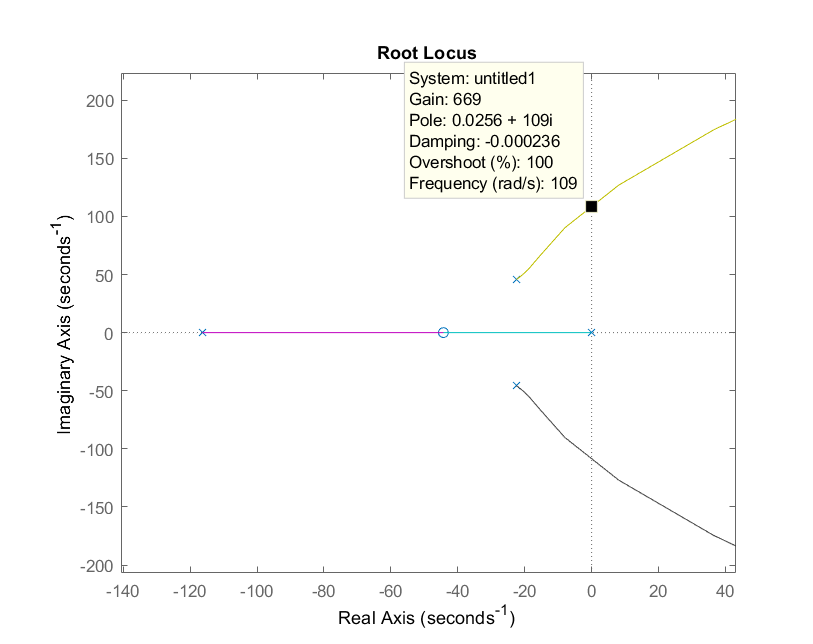
\includegraphics[scale=0.5]{rlocusconintegrador30kg.png}
	\caption{Lugar de raíces con realimentación positiva.}
	\label{fig:lugar-de-raices-con-integrador-analog}
\end{figure}
 
\noindent En la figura \ref{fig:lugar-de-raices-con-integrador-analog} se puede observar que, para que se mantenga la estabilidad del sistema, la ganancia del integrador ($K_{int}$) debe ser menor a 669. Teniendo esto en cuenta, en la figura \ref{fig:respuesta-al-escalon-con-k-1-M-30-analog} se muestra la respuesta al escalón del sistema compensado con el integrador para una ganancia de $K_{int}=1$. Por otro lado, para obtener una salida positiva es necesario considerar el bloque F del diagrama \ref{fig:diag-externo_real_positiva} como una ganancia unitaria negativa.

\begin{figure}[H]
	\centering
	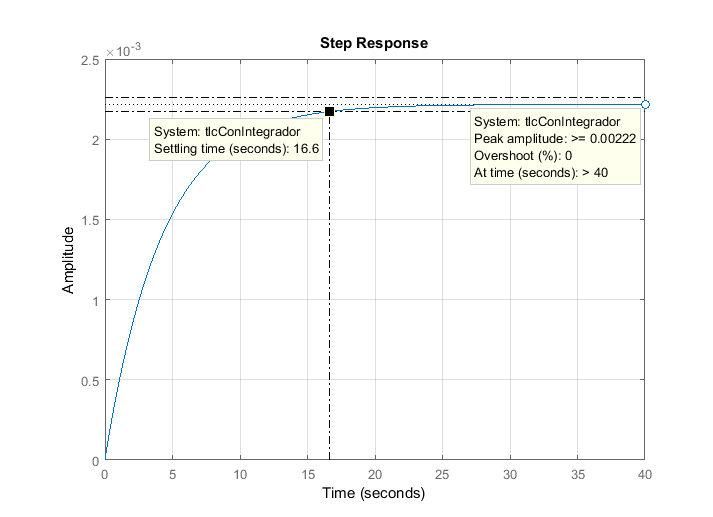
\includegraphics[scale=0.8]{stepresponseintegradorkint_1_m_30.png}
	\caption{Respuesta al escalón con integrador con $K_{int} =1$ y $M=30\:kg$.}
	\label{fig:respuesta-al-escalon-con-k-1-M-30-analog}
\end{figure}

Al observar la figura \ref{fig:respuesta-al-escalon-con-k-1-M-30-analog} es posible notar que la respuesta al escalón, si bien no posee oscilaciones, tiene un tiempo de establecimiento de aproximadamente $16.6 \:s$. Por lo tanto, para que el sistema presente mayor velocidad de respuesta, se decide aumentar el valor de ganancia hasta obtener una relación aceptable entre este tiempo y el sobrepico.



\noindent En la figura \ref{fig:respuesta-al-escalon-con-k-50-M-30}, se observa la respuesta al escalón para una ganancia del integrador de $K_{int}=50$ que resulta en un tiempo de establecimiento de $0.6\:s$ y un sobrepico de 0\%. Por lo tanto, se adopta este valor de ganancia para el diseño del integrador. Finalmente la transferencia del compensador externo queda:

\begin{equation} \label{eq_gexterno}
	G_{ext}=\frac{50}{1+\frac{s}{0.1\:r/s}}	
\end{equation}

\begin{figure}[H]
	\centering
	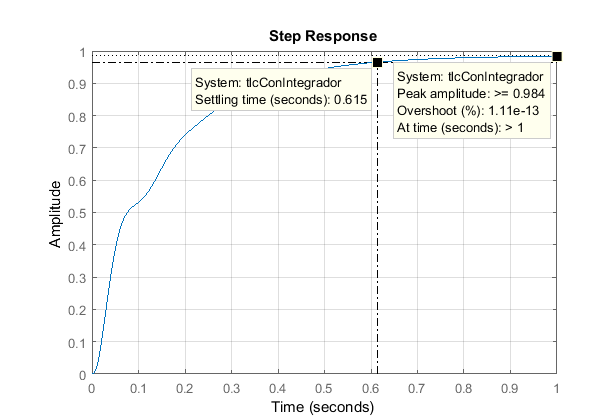
\includegraphics[scale=0.8]{stepresponseintegradorkint_50_m_30.png}
	\caption{Respuesta al escalón con integrador para $K_{int}=50$ y $M = 30\:kg$.}
	\label{fig:respuesta-al-escalon-con-k-50-M-30}
\end{figure}

\noindent La respuesta al escal\'{o}n cuando la masa es de $1 \:kg$ se muestra en la figura \ref{fig:respuesta-al-escalon-con-k-50-M-1}. All\'{i} se puede observar que el tiempo de establecimiento es de $0.74\:s$ y que no presenta sobrepicos.

\begin{figure}[H]
	\centering
	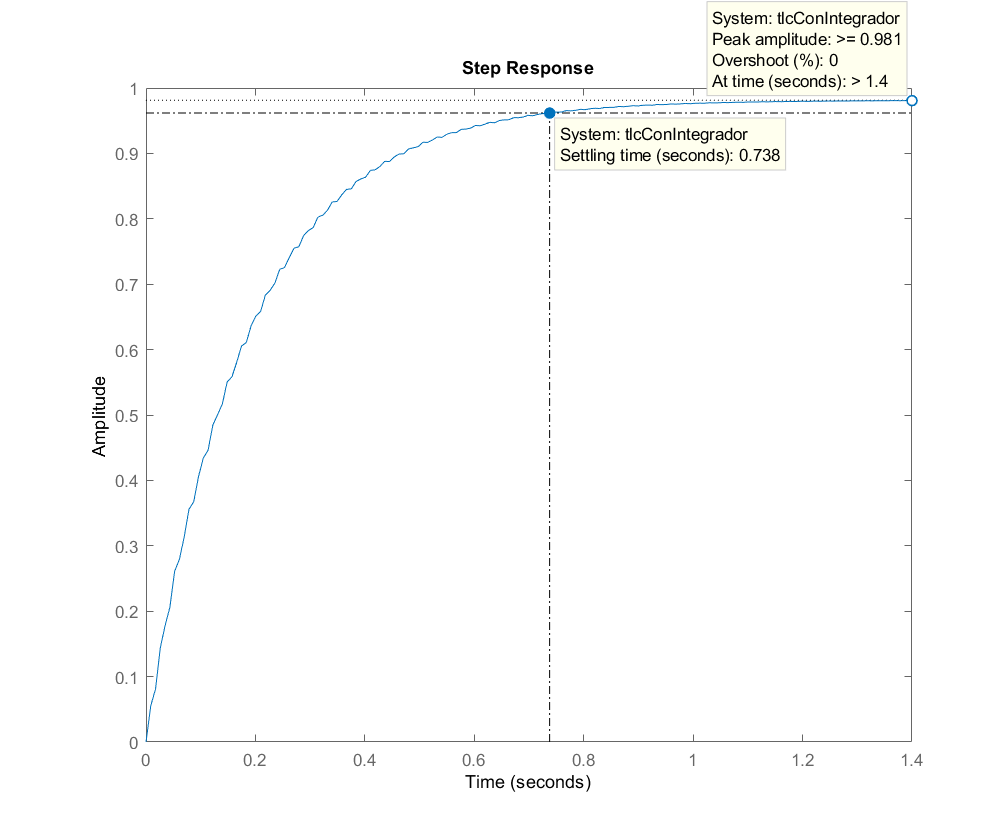
\includegraphics[scale=0.85]{stepresponseintegradorkint_50_m_1.png}
	\caption{Respuesta al escalón con integrador para $K_{int} =50$ y $M = 1 \:kg$.}
	\label{fig:respuesta-al-escalon-con-k-50-M-1}
\end{figure}


\section{Cálculo de ganancia de entrada F} \label{sec_calculo_F}

Para que la tensión de referencia de posición $V_{y_{ref}}$ se corresponda con el valor deseado de distancia de entrehierro $Y_g$ se utiliza el bloque nombrado F en la figura \ref{fig:diag-externo_real_positiva}. 

Como se vio en la sección \ref{seccopn-estim-completo} la salida del estimador para cada valor de posición toma los  valores mostrados en la tabla \ref{tab_Resultados_de_simulación_del_estimador}. Estos fueron obtenidos a partir de la siguiente ecuación:

\begin{equation}
	V_{estim}=Y_g*H_{estim}+3.4V
\end{equation}


Por lo tanto, se utilizan los mismos valores de $V_{estim}$ para la tensión de entrada $V_{y_{ref}}$. De esta forma, se obtiene la tabla \ref{tension-ref-vs-separacion-deseada}.

\begin{table}[H]
	\begin{center}
		\begin{tabular}{| c | c |}
			\hline
			$Y_{g_{deseado}}\:[mm]$ & $V_{y_{ref}}[V]$\\ \hline
			2 &	3.92 \\ \hline
			3 & 4.18\\ \hline
			4 & 4.44 \\ \hline
			5 & 4.7\\ \hline
		\end{tabular}
		\caption{Tensión de referencia $[V_{y_{ref}}]$ Vs separación deseada [$Y_g$].}
		\label{tension-ref-vs-separacion-deseada}
	\end{center}
\end{table}

En la compensación del lazo externo se utiliza un controlador con un polo en baja frecuencia, que si bien se aproxima como un integrador para la planta, no genera un error nulo en régimen permanente. Por lo tanto, se producirá una diferencia en la posición de salida $Y_g$ con respecto a la deseada según la tensión de referencia  $V_{y_{ref}}$. 

Para lograr que no haya diferencia entre la posición de salida y la deseada se debe elegir un valor de ganancia adecuado para el bloque F. Su correcta elección permite que este error sea nulo para un determinado valor de tensión de referencia de posición en la entrada. Por lo tanto, se decide diseñar el bloque F para eliminar el error para una posición de salida $Y_g=4\:mm$.

Para calcular el valor de F adecuado se debe obtener el valor en régimen permanente de la señal $V_{e_{ext}}$ mostrada en el diagrama de la figura \ref{fig:lugar-de-raices-con-integrador-analog}. Este puede ser calculado como:

\begin{equation} \label{eq_veext_ss}
	Ve_{ext_{ss}}=\frac{V_{y_{ref}}*F}{1-k_p}
\end{equation}

Donde: 

\begin{equation*}
	k_p=\lim\limits_{s \to 0}[G_{ext}(s)*TLC_{interna}(s)*H_{estim}(s)]=-67.78
\end{equation*}

La señal $Ve_{ext}$ puede calcularse como:

\begin{equation} \label{eq_veext_2}
	Ve_{ext}=V_{y_{ref}}*F+V_{estim}
\end{equation}

Entonces, al diseñar F tal que la salida para $4\:mm$ coincida con el valor en la referencia ($V_{y_{ref}}=4.44\:V$), resulta  $V_{estim}=4.44\:V$. A partir de las ecuaciones \ref{eq_veext_ss} y \ref{eq_veext_2} se plantea:

\begin{equation}
	V_{y_{ref}}*F+V_{estim}=\frac{V_{y_{ref}}*F}{1-k_p}
\end{equation}

Al despejar el valor de F se obtiene:

\begin{equation}
	F=-\frac{V_{y_{ref}}}{V_{estim}}*\frac{1}{1-\frac{1}{1-k_p}}=-1.015
\end{equation}


En la tabla \ref{tension-ref-vs-separacion-real} se muestra el valor de salida $Y_{g_{real}}$ obtenido para cada valor de $V_{y_{ref}}$ en la entrada. Estos valores fueron calculados utilizando el software MATLAB para no perder precisión en las cifras decimales.

Los valores de $V_{estim}$ y $Y_{g_{real}}$ fueron calculados como:

\begin{equation}
	V_{estim}=V_{y_{ref}}*F*(\frac{1}{1-k_p}-1)
\end{equation}

\begin{equation}
	Y_{g_{real}}=\frac{V_{estim}-3.4\:V}{H{estim}(s=0)}
\end{equation}

\begin{table}[H]
	\begin{center}
		\begin{tabular}{| c | c | c | c |}
			\hline
			$Y_{g_{deseado}}\:[mm]$ & $V_{y_{ref}}[V]$& $V_{estim}[V]$& $Y_{g_{real}}\:[mm]$\\ \hline
			2 &	3.92 & 3.9200 & 2.0031 \\ \hline
			3 & 4.18 & 4.1800 & 3.0046\\ \hline
			4 & 4.44 & 4.4400 & 4.0062 \\ \hline
			5 & 4.7 & 4.700 & 5.0077\\ \hline	
		\end{tabular}
		\caption{Valores de distancia de entrehierro a la salida $Y_{g_{real}}$ para cada valor de tensión de referencia $[V_{y_{ref}}]$.}
		\label{tension-ref-vs-separacion-real}
	\end{center}
\end{table}

De la tabla \ref{tension-ref-vs-separacion-real} se puede ver que los valores de distancia de entrehierro real tienen una diferencia menor al $1\%$ del valor deseado.



%La realimentación tiene un punto de operación de $3.4\:V$. Por lo tanto, se le suma a $V_{y_{ref}}$ el mismo valor.
\section{Transferencia de lazo cerrado externo}

Finalmente se puede expresar la función transferencia del lazo de control externo como:

\begin{equation}
	TLC_{externa}(s)=\frac{Y_g}{V_{y_{ref}}}=\frac{F*G_{ext}*TLC_{interna}}{1-G_{ext}*TLC_{interna}*H_{estim}}
	%	\frac{-3.6301*}{den}
\end{equation}

\begin{equation*}
\resizebox{.99\hsize}{!}
{
$
TLC_{externa}(s)=\frac{1.8423*10^6 (s+44.3)^2 (s+1000)}{(s+311.7) (s+108) (s+6.128) (s^2 + 39.85s + 3039) (s^2 + 2351s + 1.497*10^6 )}
$
}
\end{equation*}

A continuación se muestra el diagrama en bloques de la estrategia de control considerando las modificaciones realizadas en el signo de la realimentación.

\begin{figure}[H]
	\centering
	\scalebox{0.8}{\tikzset{%
	buffer/.style={
		draw,
		shape border rotate=270,
		regular polygon,
		regular polygon sides=3,
		fill=blue!20,
		node distance=2cm,
		minimum height=4em
	}
}

\tikzstyle{block} = [draw, fill=blue!20, rectangle, 
minimum height=2.5em, minimum width=3em]

%Acá se define eñ diagrama en bloques completo
\begin{tikzpicture}[auto, node distance=1cm,>=latex']
	% We start by placing the blocks
	\node [input, name=input] {};
	\node [buffer, right=of input](F){F};
	\node [sum, right of=F, node distance=1.5cm] (suma_externa) {+};
	\node [block, right=of suma_externa] (externo) {$G_{ext}$};
	\node [sum, right=of externo] (suma_interna) {+};
	\node[block, right=of suma_interna] (interno) {$G_c$};
	\node [block, right=of interno] (gil) {$G_{IL}$};
	\node [block, right=of gil] (planta) {$G_p$};
	\node [block, below=of interno] (realimentacion_interna) {$H_{estim}$};
	
	\node [block, below=2cm of externo] (realimentacion_externa) {$H_{estim}$};
%	
%	\node [block, right of=suma] (amplificador) {$A(s)$};
	\node [output, right of=planta, node distance=3cm] (output) {};
%	\node [block, below of=amplificador] (realimentacion) {$H(s)$};
%	
%	
%	% Once the nodes are placed, connecting them is easy. 
	\draw [draw,->] (input) -- node[pos=0.2]{$V_{y_{ref}}$} (F);
	\draw [draw,->] (F) -- node[pos=0.9]{$+$}(suma_externa);
	\draw [draw,->] (suma_externa) -- (externo);
	\draw [draw,->] (externo) -- node[pos=0.95]{$+$} (suma_interna);
	\draw [draw,->] (suma_interna) -- (interno);
	\draw [draw,->] (interno) -- (gil);
	\draw [draw,->] (gil) -- (planta);
	\draw [draw,->] (planta) -- node[name=y]{$Y_g$} (output);
%	\draw [draw,->] (amplificador) -- node[name=y]{$V_{deriv}$} (output);
	\draw [->] (y) |- (realimentacion_interna);
	\draw [->] (realimentacion_interna) -| node[pos=0.25]{$V_{estim}$}  node[pos=0.99]{$+$} (suma_interna);
	\draw [->] (y) |- (realimentacion_externa);
	\draw [->] (realimentacion_externa) -| node[pos=0.25]{$V_{estim}$} node[pos=0.99]{$+$} (suma_externa);
\end{tikzpicture}}
	\caption{Diagrama en bloques de estrategia de compensación finalizado.}	\label{fig:diag-en-bloques-comp_final}
\end{figure}

\section{Implementación circuital}

En esta sección se aborda el diseño circuital de la etapa de compensación planteada en el diagrama \ref{fig:diag-en-bloques-comp_final}. Se realiza el diseño en orden desde la entrada $V_{y_{ref}}$ hasta llegar al compensador del lazo interno.

\subsection{Generación de tensión de referencia de posición}

\noindent Para poder modificar la distancia de separación se ingresa al sistema con una tensión variable $V_{y_{ref}}$, que se corresponde con una posición de referencia. En el circuito, esta tensión es generada por un potenciómetro que puede ser modificado por el usuario. Para generarla se utiliza el circuito mostrado en la figura \ref{fig:etapa-de-entrada}.

\begin{figure}[H]
	\centering
	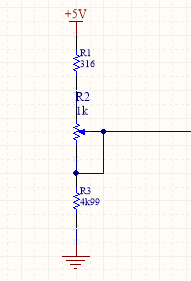
\includegraphics[scale=0.7]{Etapa-de-entrada.png}
	\caption{ Etapa de entrada.}
	\label{fig:etapa-de-entrada}
\end{figure}

Se utiliza una resistencia variable ($R_2$) de $1\:k\Omega$ y dos con valores fijos ($R_1$ y $R_3$). Para poder excursionar la tensión de referencia entre $3.92\:V$ y $4.7\:V$, los valores de las resistencias $R_1$ y $R_3$ deben ser de $4911\:\Omega$ y $313.5\:\Omega$ respectivamente. 

Por lo tanto, al adoptar un valor comercial para ellas, resulta en $R_1 = 316 \:\Omega$ y en $R_3 = 4990 \:\Omega$. De esta forma, el valor de tensión máximo para la referencia de posición queda en $4.69\:V$ y el mínimo en $3.96\:V$.

Por otro lado, se utiliza un amplificador operacional en modo seguidor de la señal $V_{r_{ref}}$ para evitar generar una carga sobre el potenciómetro. 

\subsection{Implementación circuital de la ganancia de entrada y sumador}

Como se observa en el diagrama en bloques de la figura \ref{fig:diag-en-bloques-comp_final}, luego de la etapa de generación de $V_{y_{ref}}$ se encuentra una etapa de ganancia, representada por el bloque F, junto con la suma de la señal realimentada $V_{estim}$. Este circuito estará implementado a partir de la utilización de amplificadores operacionales alimentados con fuente simple de $5\:V$, al igual que en el resto de las etapas. Es por ello que se debe tener la consideración de que la salida de esta etapa tenga un punto de operación de $2.5\:V$. Por lo tanto el circuito debe implementar la función:

\begin{equation*} 
	Ve_{ext}= 2.5\:V + V_{estim} + F*V_{y_{ref}}
\end{equation*}

Como se analizó en la sección \ref{sec_calculo_F}, el valor de F es negativo. Por lo tanto, se puede reescribir la función como:

\begin{equation} \label{eq_transferencia_veext}
	Ve_{ext}= 2.5\:V + V_{estim} - \abs{F}*V_{y_{ref}}
\end{equation}

Para lograrlo se utiliza la topología circuital mostrada en la figura \ref{fig:etapa-de-entrada-sumador}.

\begin{figure}[H]
	\centering
	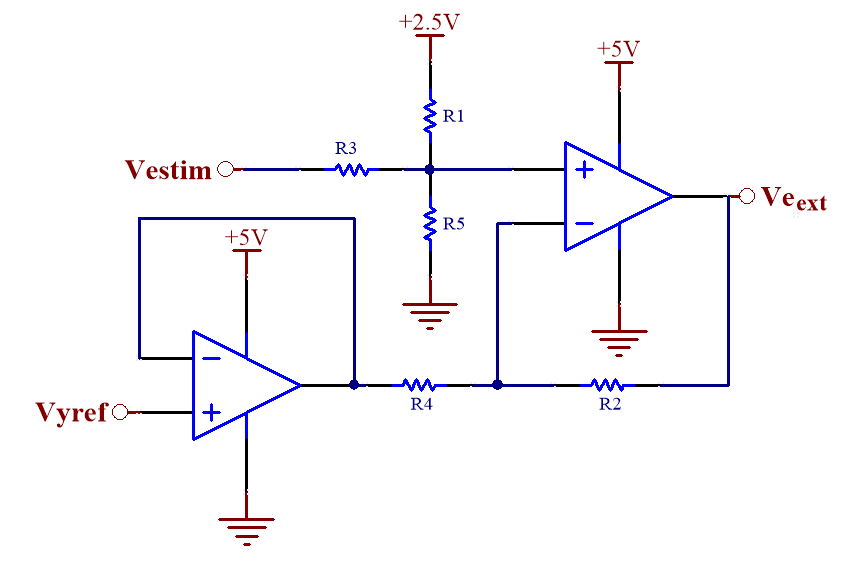
\includegraphics[scale=0.6]{Etapa-de-entrada-sumador.png}
	\caption{Circuito sumador.}
	\label{fig:etapa-de-entrada-sumador}
\end{figure}

La señal $V_{y_{ref}}$ ingresa a la entrada inversora del amplificador operacional ya que F debe ser menor que cero. Por lo tanto, a la salida del circuito se obtiene:

\begin{equation*}
	\resizebox{.99\hsize}{!}
	{
		$
		Ve_{ext}= [2.5\:V (\frac{R_3//R_5}{R_1+R_3//R_5})+V_{estim}(\frac{R_1//R_5}{R_3+R_1//R_5})](1+\frac{R_2}{R_4})-V_{y_{ref}}(\frac{R_2}{R_4})
		$
	}
\end{equation*}


Por lo tanto, al igualar los coeficientes con la ecuación \ref{eq_transferencia_veext} se obtienen las siguientes expresiones de diseño:


\begin{equation} \label{eq_relacion1}
	\frac{R_3//R_5}{R_1+R_3//R_5}*(1+\frac{R_2}{R_4})=1
\end{equation}

\begin{equation} \label{eq_relacion2}
	\frac{R_1//R_5}{R_3+R_1//R_5}*(1+\frac{R_2}{R_4})=1
\end{equation}

\begin{equation} \label{eq_relacion3} 
	\frac{R_2}{R_4}=\abs{F}=1.015
\end{equation}

Al igualar la expresión \ref{eq_relacion1} y \ref{eq_relacion2}, y reemplazar con \ref{eq_relacion3}, se obtiene:

\begin{equation*} 
	R_1 = R_3
\end{equation*}

\begin{equation*} 
	R_6=\frac{R_1*R_3}{R_1*1.015-R_3}
\end{equation*}

Se elije $R_1=R_3=1\:k\Omega$, resultando en $R_6=66.7\:k\Omega$.

Para obtener el valor de $F=1.015$ a partir del cociente entre  $R_2$  y $R_4$, se utilizan resistencias de $1015\:\Omega$ y $1000\:\Omega$, respectivamente.

\subsection{Implementación circuital del integrador}

Para implementar la transferencia de $G_{ext}$ (calculada en \ref{eq_gexterno}) se utiliza un circuito basado en un amplificador operacional. Este tiene una red de realimentación RC para que su transferencia de lazo cerrado tenga el polo del compensador. Como se utiliza un amplificador operacional con alimentación simple de $5\:V$, se desea que la salida tenga un punto de operación de $2.5\:V$. Por lo tanto, se implementa la función:

\begin{equation}
	V_{ref_c}=2.5\:V+V_{e_{ext}}*\frac{K_{int}}{1+\frac{s}{p_{int}}}
\end{equation}

\noindent En la figura \ref{fig:circuito-integrador} se puede observar la topología utilizada para el diseño del circuito integrador.

\begin{figure}[H]
	\centering
	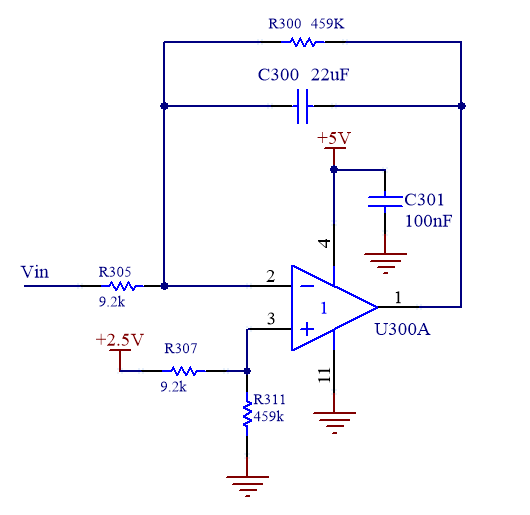
\includegraphics[scale=0.6]{Circuito-integrador.png}
	\caption{Implementación circuital del integrador.}
	\label{fig:circuito-integrador}
\end{figure}

A continuación se plantea cómo está formada la salida del circuito con respecto a cada una de sus entradas. Para simplificar la escritura de las ecuaciones se define $X_{300}$ como la relación entre el paralelo de $R_{300}$ y la reactancia de $C_{300}$ y $\tau 0 = R_{300}*C_{300}$:

\begin{equation}
	X_{300} = R_{300} // \frac{1}{s*C_{300}} = \frac{R_{300}}{1+s*\tau 0}
\end{equation}

La salida del circuito de la figura está dada por:

\begin{equation} \label{eq_salida_integrador}
	V_{ref_c}=2.5\:V*\frac{R_{311}}{R_{307}+R_{311}}*(1+\frac{X_{300}}{R_{305}})-V_{e_{ext}}*\frac{X_{300}}{R_{305}}
\end{equation}

Si se considera que la tensión de $2.5\:V$ en la entrada no inversora es continua, se puede considerar que el término de $X_{300}$ es constante con valor $R_{300}$. Por lo tanto se puede reescribir la ecuación \ref{eq_salida_integrador} como:

\begin{equation} \label{eq_salida_integrador_2}
	V_{ref_c}=2.5\:V*\frac{R_{311}}{R_{307}+R_{311}}*(1+\frac{R_{300}}{R_{305}})-V_{e_{ext}}*\frac{R_{300}}{R_{305}}*\frac{1}{1+s*\tau 0}
\end{equation}

De \ref{eq_salida_integrador_2} se plantean tres ecuaciones de diseño:

\begin{equation} \label{eq_polo_integrador}
	\frac{1}{1+s*\tau 0}=\frac{1}{1+\frac{s}{p_{int}}}
\end{equation}

\begin{equation} \label{eq_ganancia_integrador}
	\frac{R_{300}}{R_{305}}=50
\end{equation}


\begin{equation} \label{eq_ganancia_vop_integrador}
	2.5\:V*\frac{R_{311}}{R_{307}+R_{311}}*(1+\frac{R_{300}}{R_{305}})=2.5\:V
\end{equation}

Se comienza con el diseño del polo del circuito utilizando la ecuación \ref{eq_polo_integrador} y se obtiene:

\begin{equation}
	R_{300}*C_{300}=\frac{1}{0.1r/s}
\end{equation}

Se elige el valor del componente $C_{300}=22\:\mu F$, lo que resulta en $R_{300}=454.5k\:\Omega$, que se aproxima al valor comercial mas cercano $R_{300}=459\:k\Omega$.

Luego se resuelve la ecuación \ref{eq_ganancia_integrador} para obtener el valor de $R_{305}=9.18\:k\Omega$, que se aproxima al valor comercial $R_{305}=9.2\:k\Omega$.

Finalmente se resuelve la ecuación \ref{eq_ganancia_vop_integrador} para obtener la relación $R_{307}=50*R_{311}$. Por lo tanto se elige $R_{311}=9.2\:k\Omega$ y se obtiene $R_{307}=459\:k\Omega$.


Con este circuito se obtiene la función transferencia del compensador, sin considerar el punto de operación:

\begin{equation} \label{eq_gexterno_circuito}
	G_{ext_{circuito}}=-\frac{50}{1+\frac{s}{0.1r/s}}
\end{equation}

Es importante notar que la transferencia del circuito agrega una inversión de signo que no se encontraba presente en la transferencia del controlador diseñado,. Por lo tanto, debe cancelarse este signo en la siguiente etapa, que corresponde al sumador del lazo de realimentación interno.


\subsection{Etapa sumador lazo interno}

Una vez obtenida la salida del compensador externo, esta ingresa a un sumador con la señal de realimentación, para que luego el resultado ingrese al lazo de control interno.

En el diagrama en bloques de la figura \ref{fig:diag-en-bloques-comp_final} esta señal ingresa al sumador con signo positivo. Sin embargo, en la etapa anterior se generó una inversión de signo que no estaba contemplada en el diagrama en bloques. Es por ello que se decide utilizar esta etapa de sumador para cancelar dicha inversión. Además, debido a que se utiliza un amplificador operacional alimentado con fuente simple, también se agrega el punto de operación de $2.5\:V$ en la salida. Por lo tanto, la función que se debe implementar es:

\begin{equation}
	Ve_{int}=2.5\:V+V_{estim}-V_{ref_c}
\end{equation}

El circuito utilizado para implementar la función se muestra en la figura \ref{fig:circuito-sumador-lazo-interno}. 

\begin{figure}[H]
	\centering
	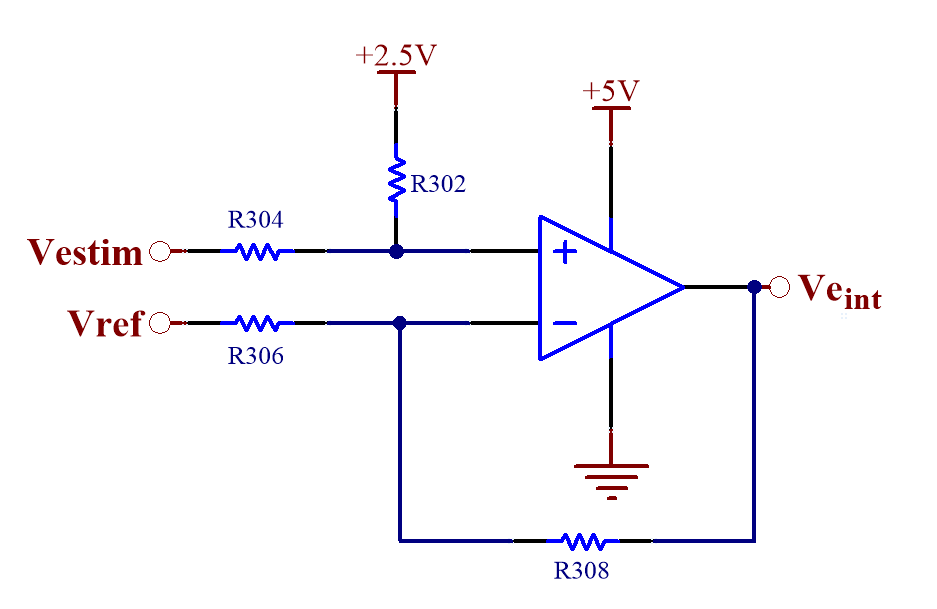
\includegraphics[scale=0.5]{Circuito_sumador_lazo_interno.png}
	\caption{Sumador del lazo interno.}
	\label{fig:circuito-sumador-lazo-interno}
\end{figure}

Para que este circuito genere correctamente la función deseada, se analiza su salida en función de sus componentes:

\begin{equation*}
	Ve_{int}=2.5\:V*\frac{R_{304}}{R_{304}+R_{302}}*(1+\frac{R_{308}}{R_{306}})+V_{estim}*\frac{R_{302}}{R_{304}+R_{302}}*(1+\frac{R_{308}}{R_{306}})-V_{ref_c}*\frac{R_{308}}{R_{306}}
\end{equation*}

Al igualar los coeficientes con la ecuación \ref{fig:circuito-sumador-lazo-interno} se pueden plantear las siguientes ecuaciones de diseño:

\begin{equation}
	\frac{R_{308}}{R_{306}}=1
\end{equation}

\begin{equation}
	\frac{R_{304}}{R_{304}+R_{302}}*(1+\frac{R_{308}}{R_{306}})=1
\end{equation}

\begin{equation}
	\frac{R_{302}}{R_{304}+R_{302}}*(1+\frac{R_{308}}{R_{306}})=1
\end{equation}

Al resolver este conjunto de ecuaciones se obtiene que todas las resistencias deben tener el mismo valor. Por lo tanto, se elige que todas sean de $1\:k\Omega$.

\subsection{Compensador interno}

En esta sección se realizará el diseño del compensador del lazo de control interno. Este puede ser dividido en tres etapas internas: dos redes de adelanto de fase conectadas en cascada seguidas de una ganancia.

A continuación se realiza el diseño de cada una de las etapas internas por separado.

\subsubsection{Implementación circuital de la red de adelanto de fase}

Para cada red de adelanto de fase se utiliza la topología mostrada en la figura \ref{fig:red-adelanto-fase}. Se desea obtener una transferencia como la calculada en \ref{eq_tf_adelanto}. A continuación se analiza el circuito propuesto y se determinan los valores de cada componente. 
%Consiste en  un polo y un cero con ganancia unitaria (si $R_a = R_b$). Luego, se agrega la ganancia como una etapa separada.

\begin{figure}[H]
	\centering
	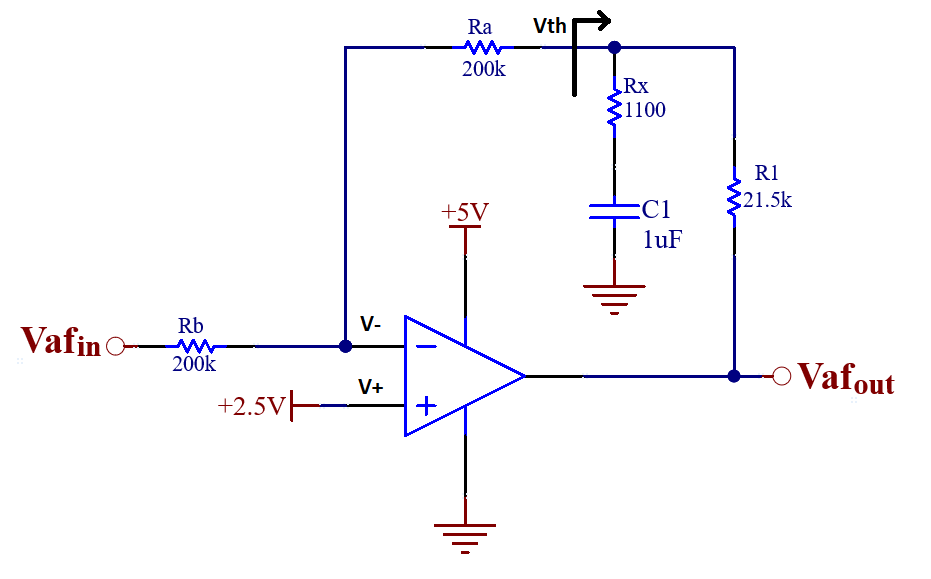
\includegraphics[scale=0.55]{Red-adelanto-fase.png}
	\caption{Diseño circuital de una red de adelanto de fase.}
	\label{fig:red-adelanto-fase}
\end{figure}

Para realizar el análisis se debe obtener los bloques de avance ($A_w$) y realimentación ($H$) mostrados en la figura \ref{fig:diag-diagrama_lazo_compensador} que corresponden a:


\begin{equation} 
	H = \frac{V_d}{V_af_{out}}=\frac{V^+ - V^-}{Vaf_{out}}
	\label{eq:h_del_compensador}
\end{equation} 

\begin{equation} 
	G^- = \frac{V_d}{Vaf_{in}}=\frac{V^+ - V^-}{Vaf_{in}}
	\label{eq:g_del_compensador}
\end{equation}

\begin{figure}[H]
	\centering
	\tikzset{%
	buffer/.style={
		draw,
		shape border rotate=270,
		regular polygon,
		regular polygon sides=3,
		fill=blue!20,
		node distance=2cm,
		minimum height=4em
	}
}

\tikzstyle{block} = [draw, fill=blue!20, rectangle, 
minimum height=2.5em, minimum width=3em]

%Acá se define eñ diagrama en bloques completo
\begin{tikzpicture}[auto, node distance=2.5cm,>=latex']
	% We start by placing the blocks
	\node [input, name=input] {};
	\node [block, right=of input](F){$G^-$};
	\node [sum, right of=F, node distance=2cm] (suma_interna) {+};
	\node [block, right=of suma_interna] (interno) {$A_{w}$};
	%\node [block, right=of interno] (tlc_interna) {$TLC_{interna}$};
	\node [block, below=of interno] (realimentacion_interna) {$H$};
	
	
%	\node [block, right of=suma] (amplificador) {$A(s)$};
	\node [output, right of=tlc_interna, node distance=3cm] (output) {};
%	\node [block, below of=amplificador] (realimentacion) {$H(s)$};
%	
%	
%	% Once the nodes are placed, connecting them is easy. 
	\draw [draw,->] (input) -- node[pos=0.2]{$Vaf_{in}$} (F);
	\draw [draw,->] (F) --  node[pos=0.9]{$+$}(suma_interna);
	\draw [draw,->] (suma_interna) -- node{$V_d$} (interno);
	%\draw [draw,->] (interno) -- node{$V_{ref_c}$} (tlc_interna);
	\draw [draw,->] (interno) -- node[name=y]{$Vaf_{out}$} (output);
%	\draw [draw,->] (amplificador) -- node[name=y]{$V_{deriv}$} (output);
	\draw [->] (y) |- (realimentacion_interna);
	\draw [->] (realimentacion_interna) -| node[pos=0.25]{}  node[pos=0.99]{$-$} (suma_interna);
%	\draw [->] (y) |- (realimentacion_externa);
%	\draw [->] (realimentacion_externa) -| node[pos=0.25]{$V_{estim}$} node[pos=0.99]{-} (suma_externa);
\end{tikzpicture}
	\caption{Diagrama en bloques interno del lazo del compensador.}	
	\label{fig:diag-diagrama_lazo_compensador}
\end{figure}

Para obtener estas ecuaciones se plantea un circuito de Thevening equivalente en el nodo $V_{th}$ mostrado en la figura \ref{fig:red-adelanto-fase} obteniéndose su $V_{th}$ y $R_{th}$.

\begin{equation} 
	V_{th} = Vaf_{in}= \frac{SC_xR_x+1}{SC_x[R_1+R_x]+1}
\end{equation}

\begin{equation} 
	R_{th} = R_1 //[R_x+(\frac{1}{SC_x})]
\end{equation}

Luego se resuelve el circuito obteniendo las transferencias mostradas en las ecuaciones \ref{eq:h_del_compensador} y \ref{eq:g_del_compensador}. Por lo tanto, se obtiene:

\begin{equation} 
	H = \frac{SC_xR_x+1}{SC_x[R_1+R_x]+1} * \frac{R_b}{R_a + R_b + R_{th}}
\end{equation}

\begin{equation} 
	G^- = - \frac{R_a + R_{th}}{R_a + R_b + R_{th}}
\end{equation}

Si se considera que $Ra>>R_{th}$ estas ecuaciones se pueden reducir a: 

\begin{equation} 
	H = \frac{SC_xR_x+1}{SC_x[R_1+R_x]+1} * \frac{R_b}{R_a + R_b}
\end{equation}

\begin{equation} 
	G^- =- \frac{R_a}{R_a + R_b}
\end{equation} 
  
Si se diseña el bloque $H$ de forma tal de que $A_w>>1/H$ sea mayor en la banda de interés se puede aproximar la salida a $1/H$. De esta forma  asignando los polos y la ganancia de la ecuación \ref{eq:transferencia-del-compensador} se obtiene que:

\begin{equation} 
	\frac{R_b}{R_a+R_b}= 1 
\end{equation}

\begin{equation} 
	\frac{1}{C_x R_x} =  902.1
\end{equation} 

\begin{equation} 
	\frac{1}{C_x [R_x + R_1]} = 44.3
\end{equation} 

En la figura \ref{fig:bode_compensador_cadena_avance} se muestra el diagrama de bode del bloque $A_w$ y $1/H$.
 
\begin{figure}[H]
	\centering
	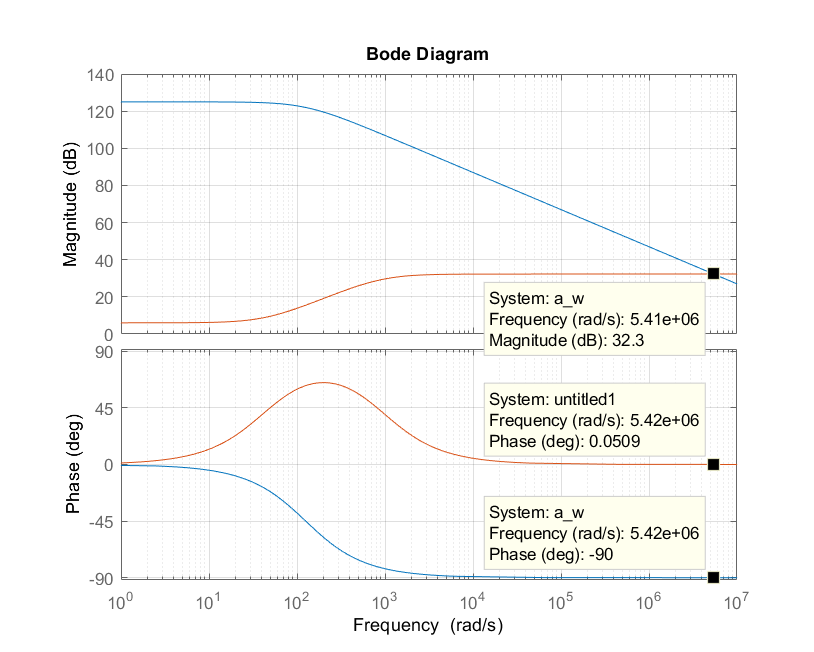
\includegraphics[scale=0.6]{bode_compensador_cadena_avance.png}
	\caption{Lazo de realimentación.}
	\label{fig:bode_compensador_cadena_avance}
\end{figure}
\colorbox{red}{aca no dije nada de la estabilidad capaz se puede decir algo aunque no sume mucho Xd tipo mfase=90 grados q opinan?}
Como se puede ver el $A_w >> 1/H$ en la banda de interes. Finalmente aproximando la transferencia de lazo cerrado interna $TLC_{af}$ a $1/H$ y multiplicando la entrada por el bloque $G^-$ se obtiene una transferencia:

\begin{equation} 
	TLC_{af} = G^- * \frac{1}{H}  =- \frac{R_a}{R_b} * \frac{SC_x[R_1+R_x]+1}{SC_xR_x+1}=-\frac{\frac{s}{44.3}+1}{\frac{s}{902.1}+1}
\end{equation}
 

Considerando el punto de operación de $2.5V$ en la entrada no inversora se obtiene:

\begin{equation} 
	Vaf_{out}= 2.5\:V* (1+\frac{R_a}{R_b})- Vaf_{in}*\frac{R_a}{R_b}*\frac{1+sC(R_x+R_1)}{1+sCR_x}
\end{equation}

Por lo tanto, para tener un polo en $902.1\:Hz$ y un cero en $44.3\:Hz$, al elegir un capacitor $C = 1\:uF$, resulta en $R_x = 1100\:\Omega$ y $R_1 = 21.5\:k\Omega$. Además, se elige $R_a = R_b = 200\:k\Omega$ para obtener una ganancia unitaria. 

\subsubsection{Ganancia de compensador interno}

La ganancia del compensador se obtiene con una etapa amplificadora por medio de un circuito como el que se muestra en la figura \ref{fig:ganancia-compensador}.

\begin{figure}[H]
	\centering
	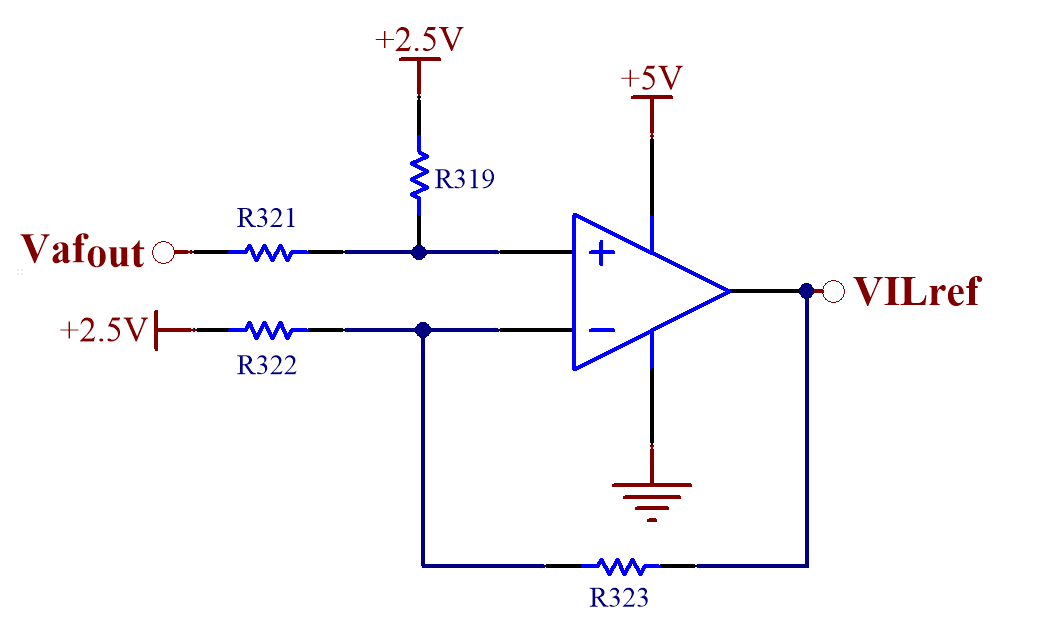
\includegraphics[scale=0.5]{Ganancia-compensador.png}
	\caption{Etapa de ganancia del compensador.}
	\label{fig:ganancia-compensador}
\end{figure}

Una de las entrada al circuito es señal $Vaf_{out}$, que está compuesta por un termino de alterna $\hat{Vaf_{out}}$ superpuesta a un punto de operación de $2.5\:V$ ($\overline{Vaf_{out}}$). Por lo tanto, debido a que solo se desea amplificar el termino de alterna, se agrega en la entrada inversora del amplificador operacional una señal que elimine dicho punto de operación. Además, como se utiliza una fuente de alimentación simple para el circuito, se desea que la salida tenga un punto de operación de $2.5\:V$. Por lo tanto, la función a implementar resulta:

\begin{equation} \label{eq_sum_int_1}
	V_{IL_{ref}}=2.5\:V+10*\hat{Vaf_{out}}
\end{equation}

La salida del circuito de la figura \ref{fig:ganancia-compensador} en función de sus entradas es:

\begin{equation}\label{eq_sum_int_2}
	\resizebox{.8\hsize}{!}
	{
		$
		V_{IL_{ref}}=(2.5\:V\frac{R_{321}}{R_{321}+R_{319}}+Vaf_{out}\frac{R_{319}}{R_{321}+R_{319}})(1+\frac{R_{323}}{R_{322}})-2.5\:V\frac{R_{323}}{R_{322}}
		$
	}
\end{equation}

Por lo tanto, a partir de las expresiones \ref{eq_sum_int_1} y \ref{eq_sum_int_2} surgen las siguientes ecuaciones de diseño:

\begin{equation}
	\frac{R_{323}}{R_{322}}=10
\end{equation}

\begin{equation} 
	(\frac{R_{321}}{R_{321}+R_{319}})*(1+\frac{R_{323}}{R_{322}}) = 1
\end{equation}

\begin{equation} 
(\frac{R_{319}}{R_{321}+R_{319}})*(1+\frac{R_{323}}{R_{322}}) = 10
\end{equation}

Para lograr una ganancia de $10$ se elige $R_{322} = 1\:k\Omega$ y resulta $R_{323} = 10\:k\Omega$. Luego, resolviendo el resto de ecuaciones se llega a $R_{319}=10\:k\Omega$ y $R_{321}=1\:k\Omega$.

Finalmente en la figura XD se muestra el circuito de todas las etapas del compensador interno en cascada para obtener de esta forma la transferencia mostrada en la ecuación \ref{eq:transferencia-del-compensador}

\colorbox{red}{Agregar imagen con las dos redes y la ganancoa, la señal de entreda es Veint}

\colorbox{red}{Hacer bode de la red de adelanto de fase con NL5 o ver de simularlo de alguna otra manera}